% ###################################################################################################
%
%  Documentation:   DichroCalc 
%
%  Author:          Benjamin M. Bulheller
%
%  Affiliation:     Research group Jonathan D. Hirst
%                   University of Nottingham, UK
%
%                   Research group Shaul Mukamel
%                   University of California at Irvine, USA
%
%  Version:         $Revision: 4621 $, $Date: 2009-07-06 09:11:08 +0100 (Mon, 06 Jul 2009) $
%
%  Date:            May 2009
%
% ###################################################################################################

\documentclass[11pt, letterpaper]{article}

\usepackage{graphicx}
\usepackage{amsmath}
\usepackage{mathdots}
\usepackage{booktabs}
\usepackage{multirow}
\usepackage{rotating}
\usepackage{xspace}
\usepackage{color}
\usepackage[superscript]{cite}    % to format the citation-format (citeleft, citeform, citeright)
\usepackage[top=2cm, bottom=2cm, left=2.5cm, right=2.5cm]{geometry}

\newcommand{\colred}  [1] {\textcolor{red}{#1}}
\newcommand{\colblue} [1] {\textcolor{blue}{#1}}
\newcommand{\colgreen}[1] {\textcolor{green}{#1}}

\usepackage{caption}              % to manipulate the caption width
\captionsetup{width=0.8\textwidth, labelformat=simple, labelsep=colon}

\setlength{\parskip}{1em}
\setlength{\parindent}{0em}

% \setcounter{secnumdepth}{-2}

\newcommand{\tab}{\hspace{0.7cm}}
\newcommand{\dotbar}{{\scriptsize$\vdots$}\hspace{-0.7ex}}
\newcommand{\Endangle}{\raisebox{0.55ex}{\scriptsize \textsf{L}}}

\newcommand{\npi} {$n\rightarrow\pi^*$\xspace}
\newcommand{\pipi}{$\pi\rightarrow\pi^*$\xspace}

\newcommand{\class}  [1]{\footnotesize\hspace{1ex}(\emph{\texttt{#1}})}
\newcommand{\atGroup}{\texttt{at(}\emph{Group}\texttt{)}}
\newcommand{\atState}{\texttt{at(}\emph{State}\texttt{)}}
\newcommand{\atTrans}{\texttt{at(}\emph{Trans}\texttt{)}}
\newcommand{\atPerm} {\texttt{at(}\emph{Perm}\texttt{)}}
\newcommand{\atType} {\texttt{at(}\emph{Type}\texttt{)}}
\newcommand{\atAtom} {\texttt{at(}\emph{Atom}\texttt{)}}
\newcommand{\atMono} {\texttt{at(}\emph{Mono}\texttt{)}}
\newcommand{\atIndex}{\texttt{at(}\emph{Index}\texttt{)}}
\newcommand{\atCoord}{\texttt{at(0|1|2)}}

% ====================================================================================================

\begin{document}

\begin{titlepage}
\begin{center}

\includegraphics[height=3.5cm]{figures/LogoPsi.eps}
\hspace{4.5cm}

\includegraphics[height=3.1cm]{figures/LogoDichroCalc.eps}

\vspace*{3.0cm}
\Huge \bf Dichroism Calculations \\

\vspace{4.0cm}

{\huge DichroCalc}

\vspace{4cm}

\Large Benjamin M.\ Bulheller

\vspace{3cm}

\enlargethispage{4em}
\normalsize

\begin{tabular}{p{8cm}p{8cm}}
\begin{center}
Research Group \\
Jonathan D.\ Hirst \\
University of Nottingham \\
Nottingham \\
United Kingdom
\end{center}
&
\begin{center}
Research Group \\
Shaul Mukamel \\
University of California \\ Irvine \\
USA
\end{center}
\end{tabular}

\end{center}
\newpage

\end{titlepage}


% ====================================================================================================


\tableofcontents

\newpage

\section{Introduction}

\subsection{General Information and Conventions}

All variables that are global within the DichroCalc object are named with the prefix \verb'DC_' to indicate their global scope. The data read from the input and parameter files are stored in nested data structures instead of multiple variables. The advantage of this is that such structures combine a lot of information in an organized fashion as opposed to data scattered over several variables. A structure can be passed on to routines as a whole and it is also available to functions outside the object. For example, \verb'DC_ParSets' contains all parsed parameter set data, \verb'DC_System' all information about the processed system, and \verb'DC_Results' all results of the calculation.

The data structures and classes used to build them are shown in detail in section \ref{Sec:ObjectStructure}. For each class \verb'X' that is defined in the class \verb'Dichro' (\verb'dichrocalc.h'), an individual function \verb'OutputXClass' was created that prints the entire variable based on the class to the \verb'.dbg' file. Dedicated output functions are important and generally recommended when defining large structures as it is otherwise not possible to output them quickly, e.g.\ during debugging. Mind that if any changes are done to the class definitions, these have to be reflected in the respective output function to avoid breaking it. The output routines generally print to the debug file because the structures often contain a large amount of data. Therefore, the \verb'-debug' option is required when such functions are used. Another advantage of using output routines for classes is that it removes the clutter of printing the content from the routines filling and processing the data structures.

The main header file containing all class and function definitions is \verb'dichrocalc.h' with the main class being \verb'class Dichro'. It is also used as central point for including header files, that is all inclusions required by other parts of the program are collected there. Therefore, \verb'dichrocalc.h' is the only header file included by other program files. It is also the interface to the outside and is the only file needed to be included by programs using DichroCalc (apart from the library which has to be linked during compilation).

In general, strings and vectors are used exclusively, disfavoring C-style strings and arrays, respectively. The only exception are variables involved in linear algebra calculations, for which the NewMat types are used and which are only accessed using the respective NewMat functions. The access to array/vector elements starts counting at 0 and, to stay consistent, for NewMat variable types the \verb'.element(row,col)' accessor function is used because it also starts counting at 0, while other access methods in NewMat~11 start at 1. Elements in vectors are accessed using the \verb'.at(row).at(col)' function because of its built-in range check (which the access using \verb'[row][col]' does not feature). In order to avoid errors, there is also no `conversion' done for output to the debug file, that is the first transition on the third group is referred to as \emph{transition 0} of \emph{state 0} on \emph{group 2}.

The standard type for floating point variables is \verb'double' throughout the program. When \verb'float' was used instead, the results showed too large deviations, and to avoid numerous casting commands, \verb'double' was chosen in general.

The web interface of DichroCalc\cite{Bulheller:09:539} offers the same possibilities for CD and LD as the command line version (in combination with the \verb'bandshape' script). To perform an orientation search while calculating the LD, the online version has to be used, which will return a PDF report for multiple orientations of the PDB.


% ----------------------------------------------------------------------------------------------------


\subsection{Files and Folder Structure}

The folder structure differs slightly between the stand-alone version, which was designed to be fully contained in one directory tree, and the version used in Spectron. The source files are identical, the differences are the makefiles, which expect the required library of NewMat in different locations, and some additional folders with information required by the Spectron makefile.

\subsubsection{Folder Structure of Stand-Alone Version}

\begin{tabular}{p{3.5cm}l}
\verb'dichrocalc/'                    &                                                                             \\
\tab \textbar  --- \verb'include/'    & all DichroCalc header files and the compiled library \verb'libdichrocalc.a' \\
\tab \textbar  --- \verb'lib/'        & third-party header files and libraries (currently only NewMat)              \\
\tab \textbar  --- \verb'obj/'        & the object files compiled from the \verb'.cpp' files                        \\
\tab \textbar  --- \verb'src/'        & \verb'.cpp' source code files of DichroCalc                                 \\
\tab \textbar                         &                                                                             \\
\tab \textbar  --- \verb'dichrocalc'  & the compiled binary for stand-alone use                                     \\
\tab \Endangle --- \verb'makefile'    & the makefile to build the binary and library                                \\
\end{tabular}


\subsubsection{Folder Structure of Spectron Version}

\begin{tabular}{p{5.5cm}l}
\verb'dichrocalc/'                                 &                                                              \\
\tab \textbar  --- \verb'dichrocalc/'              &                                                              \\
\tab \textbar  \tab \textbar  --- \verb'dep/'      & files declaring the dependencies of each source file         \\
\tab \textbar  \tab \textbar  --- \verb'doc/'      & the DichroCalc documentation                                 \\
\tab \textbar  \tab \textbar  --- \verb'include/'  & all DichroCalc header files                                  \\
\tab \textbar  \tab \textbar  --- \verb'obj/'      & the object files compiled from the \verb'.cpp' files         \\
\tab \textbar  \tab \textbar  --- \verb'src/'      & \verb'.cpp' source code files of DichroCalc                  \\
\tab \textbar  \tab \textbar                       &                                                              \\
\tab \textbar  \tab \Endangle --- \verb'makefile'  & the Spectron-based makefile to build the binary and library  \\
\tab \textbar                                      &                                                              \\
\tab \textbar  --- \verb'bin/'                     & output directory for the stand-alone binary                  \\
\tab \textbar  --- \verb'include/'                 & third-party header files (NewMat)                            \\
\tab \textbar  --- \verb'lib/'                     & the DichroCalc and NewMat libraries                          \\
\tab \textbar  --- \verb'newmat/'                  & NewMat source files to compile its library                   \\
\tab \textbar                                      &                                                              \\
\tab \textbar  --- \verb'configure'                & prepares the compilation, creates \verb'make.top'            \\
\tab \textbar  --- \verb'make.extralibs'           & include-file to compile the NewMat library                   \\
\tab \textbar  --- \verb'makefile'                 & include-file for Spectron-makefile to build the project      \\
\tab \textbar  --- \verb'make.top.in'              & include-file template with general compile settings          \\
\tab \Endangle --- \verb'make.top'                 & created from \verb'make.top.in' by the configure script      \\
\end{tabular}


\newpage


\subsubsection{Source Files}

\begin{itemize}

\item \verb'dichrocalc.h' \\
Main DichroCalc header file, contains all definitions of the object class. This is included in all files of DichroCalc to declare the \verb'Dichro::' class with its ``global'' variables, class definitions and functions.
\vspace{1em}

\item \verb'dichrocalc.cpp' \\
This is merely a front-end using the DichroCalc routines. The binary of it is the stand-alone version of DichroCalc.

\item \verb'iolibrary.cpp' and \verb'iolibrary.h' \\
A collection of general routines (e.g.\ for handling strings or printing structures) that are used by all files of DichroCalc.

\item \verb'readinput.cpp' \\
Routines for reading the input file (\verb'.inp') with the information on the system, and all parameter files (\verb'.par') specified in it. The parameter files are read from a directory given as parameter to the program.

The file also holds the class constructor and destructor.

\item \verb'fitparameters.cpp' \\
Holds routines to fit the parameters to the chromophores of the system. For each chromophore a new instance of the respective parameter set is created and the monopoles and dipole moments rotated and translated to be fitted to the chromophore's coordinates.

\item \verb'matrix.cpp' \\
Routines for setting up the Hamiltonian matrix.

\item \verb'dichroism.cpp' \\
The functions to calculate circular and linear dichroism.

\end{itemize}


% ----------------------------------------------------------------------------------------------------


\subsection{Units}

Input units\index{units}

\begin{itemize}
\item atom and moment coordinates: \AA ngstrom
\item monopole charges: $10^{-10}$ esu

Electrostatic Unit (esu)  = $\mbox{cm}^\frac{3}{2} \mbox{g}^\frac{1}{2} \mbox{s}^{-1}$ = $3.356\cdot10^{-10}$ C (= As) 

\item electric transition dipole moments: Debye
\item magnetic transition dipole moments: Bohr Magnetons
\item energy: $cm^{-1}$
\end{itemize}


% ====================================================================================================


\section{Compilation}

\subsection{Linear Algebra Extension NewMat}

\label{Sec:LinearAlgebraExtensions}

\begin{tabular}{p{0.5cm}p{6cm}p{10cm}}
 & \textbf{Directory} (stand-alone) & \verb'lib/newmat.source'  \\
 & \textbf{Directory} (Spectron)    & \verb'newmat/newmat11'    \\
 & \textbf{Version}                 & 11$\beta$                 \\
 & \textbf{Website}                 & http://www.robertnz.net/  \\
 & \textbf{Libraries required}      & ---                       \\
 & \textbf{Libraries created}       & \verb'lib/libnewmat.a'    \\
\end{tabular}

For DichroCalc itself only NewMat is needed for the diagonalization of the Hamiltonian matrix. The source directory of the stand-alone version contains the original tarball, the NewMat~11 documentation and folders with compiled versions for Mac OS (\verb'source.darwin') and Linux (\verb'source.linux'), respectively. The script \verb'copycompiled' can be used after the files were recompiled, it copies the library for the needed architecture to \verb'lib'.

Several makefiles are provided for different compilers (\verb'nm_*.mak'), if the required compiler is not preconfigured, the utility \verb'genmake' can be downloaded from the website to create a suitable makefile. Under Mac OS and using \verb'g++' the library can be compiled with

\begin{verbatim}
make -f nm_gnu.mak
\end{verbatim}

The final library is \verb'libnewmat.a' and needs to be linked as \verb'newmat' during the compilation of programs using the NewMat functions. If the file \verb'libnewmat.a' is at \verb'./lib', the command to compile a programs is

\begin{verbatim}
g++  program.cpp  -o program  -L./lib  -l newmat
\end{verbatim}

Mind that there must not be a space after \verb'-L'. The required header files (in \texttt{dichrocalc/lib/}) are
\begin{itemize}
\item \verb'newmat.h'
\item \verb'include.h'
\item \verb'myexcept.h'
\item \verb'newmatap.h'
\item \verb'newmatio.h'
\end{itemize}

The final release of v10 was tried, however, this suffered from linker errors that could not be resolved. Therefore, v11$\beta$ was chosen and worked without problems on both Mac OS and Linux.

The routines to reset the source directory for recompilation are \verb'clean', \verb'clobber', and \verb'distclean', given in increasing purging power. They are defined in \verb'Makefile.in', which needs to be given explicitly to \verb'make' since the inclusion in the actual makefile is not enough:
\begin{verbatim}
make -f Makefile.in distclean
\end{verbatim}


% ----------------------------------------------------------------------------------------------------


\newpage

\subsection{Compilation Parameters}

A \verb'makefile' is provided to compile the program. It was tested using \verb'gcc'/\verb'g++' version 4.0.1 under Mac OS 10.5 and version 3.3.1 under SuSE Linux 9.0. The single source files do not need any compiler switches, the crucial step is linking the NewMat library and header files when compiling the final binary. For the stand-alone version the required include commands are

\begin{verbatim}
{object files}  -I./lib  -L./lib  -I./include  -L./include  \
                -lnewmat  -ldichrocalc  -lm
\end{verbatim}

\paragraph{CAUTION:} Using \verb'g++' on Linux the sequence of the parameters is \emph{crucial}. The object files (\verb'.o') have to be given before the linker parameters, that is the directories to include and libraries to use. Otherwise the error messages will be about \verb'undefined reference's because the library is not linked during compilation. Several pages with error messages such as
\begin{verbatim}
obj/iolibrary.o(.text+0x7c89): In function `PrintMatrix(Matrix*)':
: undefined reference to `Matrix::element(int, int)'
\end{verbatim}
are due to linker problems and point to the NewMat library \verb'libnewmat.a'. This also occurs, for example, if the library was built for the wrong platform. In \verb'dichrocalc/lib/newmat.source' (stand-alone) and \verb'newmat/newmat11' (Spectron), the source files can be found to recompile the library. For the stand-alone version, the Linux and Mac OS libraries are precompiled and can be copied using the respective command:

\begin{verbatim}
./copycompiled linux
./copycompiled darwin
\end{verbatim}


% ====================================================================================================


% \newpage

\section{Performing a Calculation}

\subsection{Scripts and Perl Libraries}

The following Perl scripts are needed and require the listed libraries:

\begin{tabular*}{\textwidth}{@{\extracolsep{\fill}}lll}
\textbf{Scripts:}      &  \textbf{Libraries:}    &                           \\
\verb'dcinput'         & \verb'DebugPrint.pm'    & \verb'Error.pm'           \\
\verb'bandshape'       & \verb'GetBaseName.pm'   & \verb'GetParameters.pm'   \\
\verb'plotspectrum'    & \verb'ParsePDB.pm'      & \verb'ReadDichroCalc.pm'  \\
                       & \verb'ReadSpectrum.pm'  & \verb'VectorMath'         \\
\end{tabular*}

Perl scripts search the Perl library path for libraries. The above scripts additionally include the folder \verb'~/bin/perllib' and the directory of the actual script location. That is, all scripts can simply be kept in the same directory as the libraries. To store them separately on compute nodes without root access, the \verb'~/bin/perllib' directory can be used.


% ----------------------------------------------------------------------------------------------------


\subsection{Parameters and Output Files}

The binary (compiled from \verb'dichrocalc.cpp') is only a front-end for the library with the only purpose of feeding parameters given via the command line into the constructor. Therefore, the same features are available for use via the library (in Spectron) or the binary. The following parameters can be given via the command line (the respective options to contruct the object are covered in Section~\ref{Sec:InitializeingTheObject}):

%{\small
\begin{verbatim}
Usage: dichrocalc [options]

       -i , --input inputfile  filename of the input file to process (mandatory)
       -p , --params           directory with the parameter files (*.par)
       -v , --verbose          verbose output
       -d , --debug            set level of debug output to .dbg file (0-5)
            --vec              create .vec file (for absorbance/LD)
            --pol              create .pol file (transition polarizations)
            --mat              create .mat file (matrix, eigenvectors, eigenvalues)
       -h , --help, -?         usage output
\end{verbatim}
%}

If no additional files (such as \verb'.dbg', \verb'.vec', etc.) are requested, the only file that is produced by default if the CD line spectrum (\verb'.cdl'). If no parameter directory is given then \verb'~/bin/params' is used by default. At the beginning of the constructor there are several variables that define these defaults:

%{\small
\begin{verbatim}
	// Global configuration parameters
	DC_PrintCdl      = true;               // whether to print the .cdl file
	DC_PrintXyzFiles = false;              // files with atom coordinates
	DC_ParamsDefault = "/bin/params";      // $HOME is added  
\end{verbatim}
%}

These settings allow to prevent the creation of the \verb'.cdl' file (e.g.\ if the library is used via Spectron) and to change the default directory for the parameter files. The switch \verb'DC_PrintXyzFiles' triggers the creation of one file containing the original atom coordinates read from the PDB and the fitted coordinates of the parameter sets. The quickest way to compare the match of both coordinate sets is to run \verb'gnuplot' and issue a command such as
\begin{verbatim}
splot "coord-group.xyz", "coord-parset.xyz"
\end{verbatim}


% ----------------------------------------------------------------------------------------------------

\subsection{Workflow}

To calculate spectra, a PDB file of the protein is required for the 3D structure, that is the coordinates of the chromophores. The script \verb'dcinput' creates the input file for DichroCalc (\verb'.inp') from the \verb'.pdb'. The file contains all parameters for the calculation as well as the structural information of the protein (i.e.\ which atoms make up the chromophores), including all atom coordinates. DichroCalc requires only this file to run and produces, among several other optional output files, the line spectrum (gas phase spectrum). This is either \verb'.cdl' for CD, or \verb'.vec' for absorbance and LD. The script \verb'bandshape' adds bandshapes to the line spectra and \verb'plotspectrum' is used to create postscript files of the results.

Hence, for using the stand-alone version of DichroCalc for a CD calculation the basic steps are:
\begin{verbatim}
dcinput file.pdb          (=> file.inp)
dichrocalc -i file.inp    (=> file.cdl and file.vec)
bandshape file            (=> file.cd, file.ld, file.ab)
plotspectrum file.cd      (=> file.cd.ps)
\end{verbatim}

For use in Spectron, in addition to the \verb'.inp' file the respective Spectron input file is required. Please see the Spectron documentation for information on it.


% ----------------------------------------------------------------------------------------------------
 

\subsection{Input File}


\subsubsection{Creation}
\label{Sec:Creation}

The input file is created from a PDB file using the script \verb'dcinput'. For backbone-only calculations (parameters by Hirst or Woody), the script can be used on its own. For charge-transfer and/or side chain chromophores, the available parameters to use have to be defined in the file \verb'chromophores.dat', which is covered below.

\enlargethispage{1em}
{\small
\begin{verbatim}
Usage:   dcinput file1 [file2] [...] [options]

file       a .pdb file, the extension can be omitted
-v         verbose mode
-o         base name of the output file (only if a single file is processed)
-pdb       to output the renumbered pdb file (.inp.pdb) with the numbers
           referred to in the inp
-log       to output the log file (.inp.log) with error messages and warnings
-dbg       prints out debug information like the CT chromophore assignments (angles)

-nma       use NMA4FIT2 for the backbone chromophores (default)
-wdy       use NMA99WDY for the backbone chromophores
-urea      use urea chromophores instead of peptide chromophores for the backbone
-p SET     use the given parameter set for the backbone chromophores
-ct        include charge-transfer transitions

-sc        include aromatic side chain transitions of PHE, TYR and TRP
  -phe       include phenylalanine side chain group
  -tyr       include tyrosine side chain group
  -trp       include tryptophan side chain group

-scn       include non-aromatic side chain transitions of ASP, GLU, ASN and GLN
  -asp       include the aspartic acid carboxyl group
  -glu       include the glutamic acid carboxyl group
  -asn       include asparagine side chain peptide group
  -gln       include glutamine side chain peptide group

-nb        include parameters for all nucleic bases
  -ade       include adenine
  -gua       include guanine
  -cyt       include cytosine
  -thy       include thymine
  -ura       include uracil

-nap       include the naphthalenediimide chromophore
  -lnk       include the naphthalenediimide carboxy group (the linker)
  -trt       include the complete trityl group
  -trtsel    include specific phenyl rings of the trityl group, e.g. 12 or 13

-cyc       look for peptide bonds between non-successive residues
           (currently LYS-ASP with the atoms CG OD1 NZ supported)
-term      include the terminal carboxyl group
-nobb      do not include the backbone chromophores

-bbt       define the number of backbone transitions (1-4, default is 2)
-ctt       define the number of charge-transfer transitions (1-4, default is 4)
-sct       define the number of side chain transitions (1-4, default is 4)
-nbt       define the number of nucleic bases transitions (1 or 2, default is 2)

-x         x range of the spectrum, default is 150 to 250
-i         interval of the wavelength, default is 1

-trans x   To force a certain number of transitions for each parameter set
-bbtrans x Choose a particular transition for the backbone (do not confuse
           with -bbt!).
           1 = n-pi*, 2 = pi-pi*, 3 = pinb-pi*, 4 = n'-pi*
           This also sets the number of backbone transitions to 1.
-cttrans x Choose a particular transition for the charge-transfer transitions.
           1 = n1-pi*2, 2 = n2-pi*1, 3 = pinb1-pi*2, 4 = pinb2-pi*1
           For this you need a cut-down and sorted version of the monopole file!.
-chrom     To define a list of chromophores to be used from chromophores.dat.
           The local chromophore has to be given, too. That way it is possible
           to use only specific CT chromophores without having the same assigned
           to all groups (as it would be the case if only one chromophore was
           given in chromophores.dat).
-nochrom   To define a list of chromophores NOT to use from chromophores.dat.
           They WILL show up in the inp, but will NOT be assigned.

If a chromophores.dat is found in the current directory, it will be read, otherwise
it is tried to read ~/bin/chromophores.dat instead. To include side chains, charge-
transfer or nucleic bases, the respective command line parameters MUST be given,
otherwise the lines are ignored. The local chromophore from chromophores.dat can
be overridden via -nma, -wdy, etc.
\end{verbatim}
} % font size environment

\newpage

Internally, \verb'dcinput' uses the PDB parser \verb'ParsePDB.pm'\cite{Bulheller:09:539} to process each given file. To prepare the file for calculation, the following tasks are carried out:

\begin{itemize}
\item All hetero atoms (HETATM) and atoms stated as ANISOU, SIGATM and SIGUIJ are removed. Only the peptide bonds and side chains are taken into account during the calculation, hence the unneeded information would just make problems in case the maximum atom number is reached.

\item Inserted residues are removed. Often alternative residues are given in PDB files (numbered for example as residues 21 and 21A) to show that the protein exists with two different amino acids at a certain position. Only superimposed residues are affected by this and the inserted one, designated by a letter in the residue number, is removed. If both have a letter (like 21A and 21B), the second one is deleted.

\item Alternative atom locations are removed. If some atoms showed a positional deviation during the elucidation via the X-ray diffraction or NMR measurements, these alternative atom locations are sometimes included in the PDB. The parser detects the method used to indicate those alternatives and keeps only the first one. 

\item All chains, residues and atoms are renumbered to ensure a correct number scheme. The atom number will then match the line number and \verb'dcinput' will write the actual atom number into the \verb'.inp' file, while DichroCalc later on interprets this via the array index as the respective line number in the \verb'$COORDINATES' section. Therefore, a correct numbering is crucial.
\end{itemize}

The processed PDB file can be written out to \verb'.inp.pdb' by using the \verb'-pdb' option and a detailed log file can be requested with the \verb'-log' option. The logfile first of all lists all problems and warnings of the PDB parser, followed by all issues of \verb'dcinput' itself. All atom assignments are reported, e.g.\ ``4 5 7'' for a peptide group, which refers to the atom numbers (in \verb'.inp.pdb') as well as line numbers (\verb'$COORDINATES') of the C, O and N atom of the respective peptide bond. This allows to verify all assigned groups.

\verb'dcinput' will at first try to read the file \verb'chromophores.dat' in the current directory. If it is not found there, \verb'~/bin/chromophores.dat' will be read instead. The file looks similar to this:

\label{Page:ChromophoresDat}
{\small
\begin{verbatim}
     # Name     Type   Trans   Phi      Psi
     NMA4FIT2    LOC     2      0.0      0.0     # peptide bond
     CT01009A    CTR     4    180.0    180.0     # charge-transfer
     CTBE009A    CTR     4   -135.0    135.0     # charge-transfer
     CT-BE09A    CTR     4    135.0   -135.0     # charge-transfer
     CT05009A    CTR     4   -120.0    120.0     # charge-transfer
     CT-0509A    CTR     4    120.0   -120.0     # charge-transfer
     CT02009B    CTR     4   -120.0    180.0     # charge-transfer
     CT-0209B    CTR     4    120.0    180.0     # charge-transfer
     CT08009A    CTR     4   -120.0     60.0     # charge-transfer
     CT-0809A    CTR     4    120.0    -60.0     # charge-transfer
     CT03009A    CTR     4    -60.0    180.0     # charge-transfer
     CT-0309A    CTR     4     60.0    180.0     # charge-transfer
     CT31009A    CTR     4    -74.0     -4.0     # charge-transfer
     CT-3109A    CTR     4     74.0      4.0     # charge-transfer
     CTBT009B    CTR     4    -62.0    -41.0     # charge-transfer
     CT-BT09B    CTR     4     62.0     41.0     # charge-transfer
     CTAL009A    CTR     4    -48.0    -57.0     # charge-transfer
     CT-AL09A    CTR     4     48.0     57.0     # charge-transfer
     CT15009A    CTR     4    -60.0    -60.0     # charge-transfer
     CT-1509A    CTR     4     60.0     60.0     # charge-transfer
     PHECASI3    PHE     4      0.0      0.0     # phenylalanine
     TYRCASY4    TYR     4      0.0      0.0     # tyrosine
     TRPCASH1    TRP     4      0.0      0.0     # tryptophan
     ASNHIRST    ASN     4      0.0      0.0     # asparagine
     GLNHIRST    GLN     4      0.0      0.0     # glutamine
     ASP_CNVE    ASP     2      0.0      0.0     # aspartic acid
     GLU_CNVE    GLU     2      0.0      0.0     # glutamic acid
\end{verbatim}
} % the font size environment

Lines starting with a hash symbol can be used to add comments as shown in the first line. Each other line represents one parameter set from the respective \verb'.par' file. The first column states the name, which is given in the latter file as, for example, \verb'-NMA4FIT2-'. The second column defines the type of the set as local (backbone, LOC), charge-transfer (CTR), or side chain chromophore (PHE, TYR, TRP, etc.). Using the parameters \verb'-nma' (the default), \verb'-wdy' or \verb'-urea' it is possible to override the local chromophore given in \verb'chromophores.dat' and use another frequent one instead.

The third column denotes the number of transitions available for the set. The last two columns define the $\phi$ and $\psi$ angles for charge-transfer chromophores, and \verb'dcinput' uses those values to determine the best-fitting CT chromophore for any given dipeptide group. Especially for the number of transitions, \verb'dcinput' offers many options to override settings in \verb'chromophores.dat'.

Mind that the \verb'chromophores.dat' contains all parameter sets which \emph{can} be chosen from the available parameter files (the syntax of these is covered in section~\ref{Sec:MatrixMethodParameters}). However, only the backbone chromophore is included by default, if it is not overridden by an option such as \verb'-nobb'. To use the charge-transfer or side chain parameters, the switches \verb'-ct' or \verb'-sc' have to be given, respectively. Usually all needed configurations concerning which chromophores to take can be done via the \verb'dcinput' command line. The parameters of \verb'dcinput' allow a complete definition which parameters are to be used or omitted from the \verb'chromophores.dat' (e.g.\ charge-transfer, side chains and how many transitions) and how many transitions are to be used for each chromophore type. Many of these functions have been implemented to analyze the effect of the parameter sets and their transitions in detail on the SP175 protein set.\cite{Bulheller:08:1866}

The parameter sets for the calculation are stored in text files with the extension \verb'.par'. They are kept in one directory, whose location is given to DichroCalc by a parameter. Their syntax is covered in the following section.


% ----------------------------------------------------------------------------------------------------


\subsubsection{Syntax}

The input file (\verb'.inp') is formatted in blocks titled with keywords in \emph{capital} letters. \verb'$KEYWORD' marks the beginning of a block, \verb'$END' the last line of it. Empty lines and comments (beginning with \verb'#') are ignored and may be used to group or annotate the data. For indentation and separation of columns, blanks and tabs can be used. 

The \verb'$CONFIGURATION' block holds general information about the protein and some parameters to control DichroCalc. The individual variables of the class that stores the values internally are in the letter case as given below, however, the keywords are compared case-insensitively when the file is parsed.

{\small
\begin{tabular}{p{5cm}p{12cm}}
\verb'$CONFIGURATION'          &                                                   \\
\verb'   BBTrans     -1'       & To use a specific backbone transition             \\
\verb'   CTTrans     -1'       & To use a specific charge-transfer transition      \\
\verb'   Factor      4'        & Scaling factor for intensity (number of residues) \\
\verb'   MinWL       150'      & The minimum wavelength to plot                    \\
\verb'   MaxWL       250'      & The maximum wavelength to plot                    \\
\verb'$END'                    &                                                   \\
\end{tabular}
}

The values \verb'BBTrans' and \verb'CTTrans' are used to select a specific backbone or charge-transfer transition. If set to --1 (default) all transitions are used. A value of 0 would use only the first transition, 1 only the second transition, etc. If this feature is used, only a single transition can be included from the respective set, that is it is not possible to include only the 2$^{nd}$ and 3$^{rd}$ transition of a parameter set. Important for the use of \verb'BBTrans' is that the backbone parameter set has to be the first one (index 0). Also note that the transition sequence in the charge-transfer parameter sets differs and the ground state transitions have to be sorted identically before including, for example, only the $\pi_b\rightarrow\pi^*$ transition of all sets.

\verb'MinWL', \verb'MaxWL' and \verb'Factor' are only required for the post-processing of the spectra on the web interface of DichroCalc. For the actual calculation they are not needed. If no specific transitions are required, the whole \verb'$CONFIGURATION' section can be omitted for the use with Spectron or from the command line.

The \verb'$PARAMETERS' block lists all parameter set names that are to be used in the calculation. The names have to match case-sensitively the respective \verb'.par' filename in the directory with the parameter sets. Each name is followed by the number of transitions to be considered for it. The parameter sets are referred to in the \verb'$CHROMOPHORES' block by their index in this list and, for convenience, this index is given in last column.

{\small
\begin{tabular}{p{5cm}p{9cm}}
\verb'$PARAMETERS'               &                                                    \\
\verb'#  name      trans  index' &                                                    \\
\verb'   NMA4FIT2  2    # 0'     & This is a peptide bond                             \\
\verb'   CT01009A  4    # 1'     & The planar charge-transfer chromophore             \\
\verb'   CTBT009A  4    # 2'     & The $\alpha$-helical charge-transfer chromophore   \\
\verb'   CTBE009A  4    # 3'     & The $\beta$-strand charge-transfer chromophore     \\
\verb'$END'                      &                                                    \\
\end{tabular}
}

Each chromophore (e.g.\ peptide bond, charge-transfer group, aromatic side chain, etc.) is represented by a certain number of atoms. To these atoms the parameters are fitted later on. In the \verb'$CHROMOPHORES' block the type of the group on each line is defined in the first column by the index of the respective parameter set in the \verb'$PARAMETERS' block (second column in the latter). The following columns specify the atoms defining the chromophore, these numbers are the indices of the atom in the \verb'$COORDINATES' block. A peptide group, for example, is defined by the \emph{C}, \emph{O}, and \emph{N} atoms.

{\small
\begin{verbatim}
$CHROMOPHORES
#  type      atoms
#  peptide chromophores
    0          2       3       4
    0          6       7       8
    0         10      11      12
#  charge-transfer chromophores
    2          2       3       4       6       7       8
    2          6       7       8      10      11      12
$END                             
\end{verbatim}
}

In the above block, the first chromophore is of type \verb'0', which points to \verb'NMA4FIT2'\cite{Besley:99:9636} in the \verb'$PARAMETERS' section, the parameter set of a peptide bond. The chromophore is represented by atoms number 2, 3, and 4 in the \verb'$COORDINATES' section below. 

The atom coordinates in the \verb'$COORDINATES' block are read from the PDB file, that is they are \emph{xyz} coordinates in \AA ngstrom.

\begin{verbatim}
$COORDINATES
#          x          y          z      #  atom label
        -1.322      0.857     35.960    #     0 N
        -1.393      1.972     35.040    #     1 CA
        -0.359      1.932     33.910    #     2 C
        -0.671      2.170     32.740    #     3 O
         0.886      1.532     34.230    #     4 N
         1.994      1.430     33.300    #     5 CA
         1.789      0.408     32.170    #     6 C
         2.064      0.673     31.000    #     7 O
         1.207     -0.760     32.500    #     8 N
         0.931     -1.845     31.580    #     9 CA
        -0.055     -1.494     30.460    #    10 C
         0.158     -1.813     29.290    #    11 O
        -1.118     -0.739     30.800    #    12 N
        -2.153     -0.307     29.880    #    13 CA
        -1.663      0.607     28.750    #    14 C
        -2.017      0.438     27.580    #    15 O
etc...
$END
\end{verbatim}


% ----------------------------------------------------------------------------------------------------


% \newpage

\subsection{Matrix Method Parameters}
\label{Sec:MatrixMethodParameters}

For every chromophore type to be considered in the calculation an individual parameter set is required. Each set needs to be in a separate file with the same name (case-sensitive) and the extension \verb'.par'. DichroCalc takes a directory name as parameter, so usually all available parameter set files are saved in a special folder whose name is passed on to DichroCalc. The available parameters have to be defined in the file \verb'chromophores.dat', which is read by the \verb'dcinput' script while the input file for DichroCalc is created (see section \ref{Sec:Creation}).

A parameter set for matrix method calculations first of all requires a set of reference coordinates. For NMA4FIT2,\cite{Besley:99:9636} the parameters of a peptide bond, these are the atoms with the PDB labels \verb'C', \verb'O', and \verb'N'. A transition is defined by its transition energy, electric and magnetic transition dipole moment, and a set of monopole charges. The monopoles are placed near or at the atom positions of the parameter set (Figures \ref{Fig:Monopoles-Hirst} and \ref{Fig:Monopoles-Woody}). Charge-transfer parameters contain two peptide groups next to each other, both with the same monopole configuration as shown in Figure~\ref{Fig:Monopoles-Hirst}. Note that in NMA4FIT2 the hydrogen atom is not actually contained as a reference atom; only the monopoles have been fitted to the position where the hydrogen atom was in the calculations.

\begin{figure}[p]
\centering
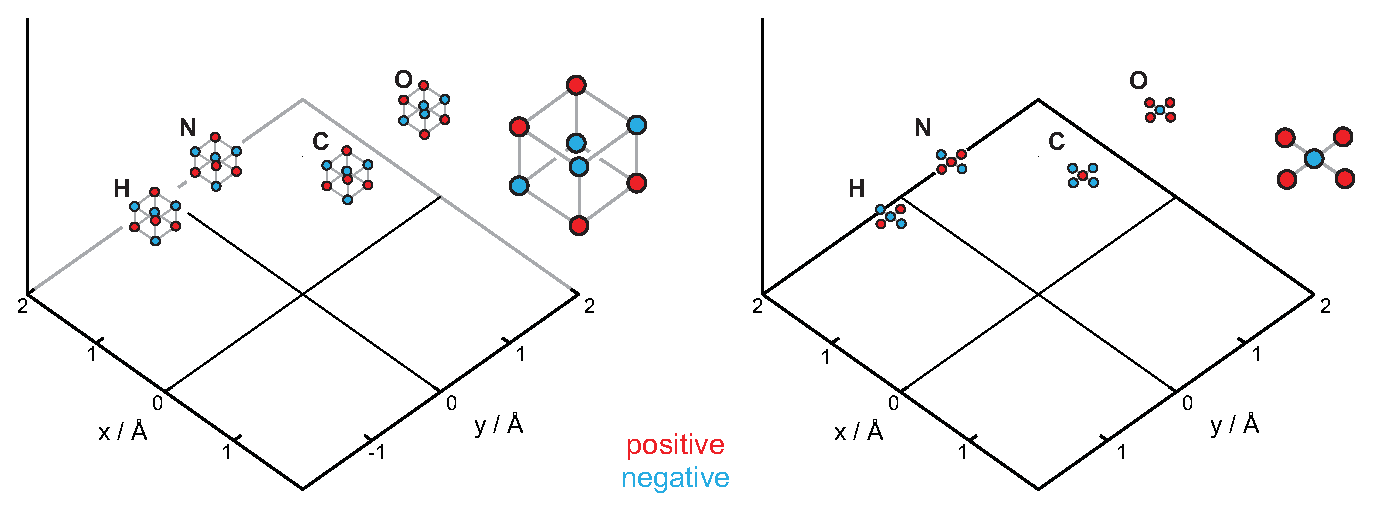
\includegraphics[width=\textwidth]{figures/monopoles-hirst.eps}
\caption{Monopole positions of the \emph{ab initio} amide parameter set, NMA4FIT2,\cite{Besley:99:9636} for the \npi transition (left panel) and the \pipi transition (right panel). Negative charges are represented by blue circles and positive charges by red circles. The distance of the monopoles to the atoms is about 0.1~\AA\ in the left panel and either 0 or 0.05~\AA\ in the right panel.}
\label{Fig:Monopoles-Hirst}
\end{figure}

\begin{figure}[p]
\centering
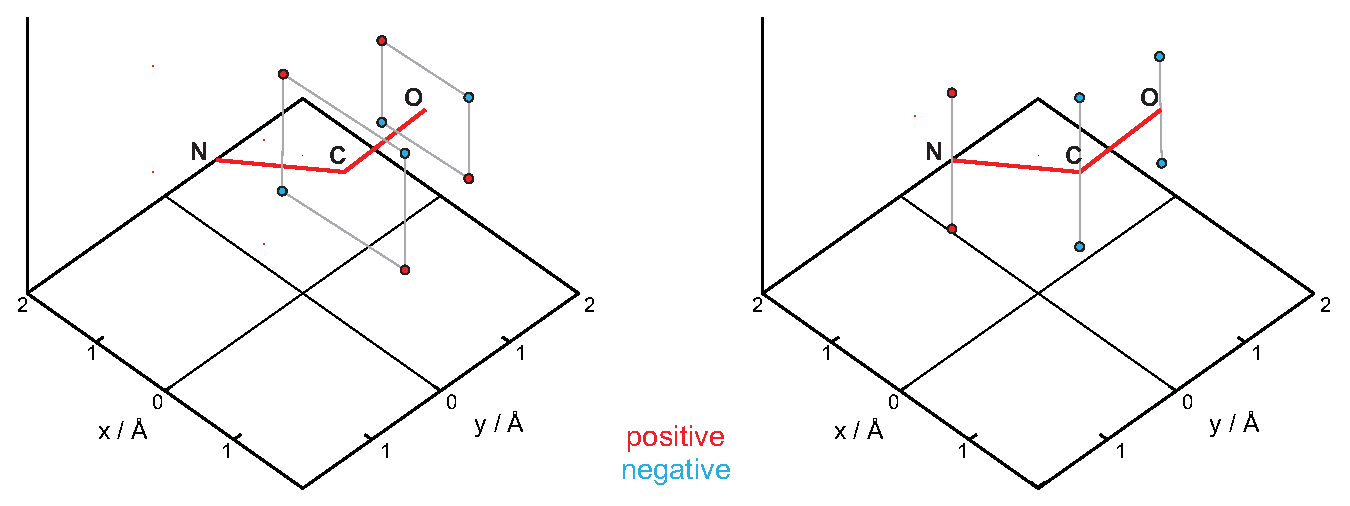
\includegraphics[width=\textwidth]{figures/monopoles-woody.eps}
\caption[Monopole positions of the semiempirical amide parameter set]
        {Monopole positions of the semiempirical amide parameter set, NMA99WDY,\cite{Woody:99:2844} for the \npi transition (left panel) and the \pipi transition (right panel). Negative charges are represented by blue circles and positive charges by red circles. The distance of the monopoles to the atoms is between 0.8 and 1.2~\AA.}
\label{Fig:Monopoles-Woody}
\end{figure}

The first line of a parameter set file must contain the name of it, identical to the filename. The second states the number of atoms to be read in. Each atom coordinate (\AA ngstrom) is followed by a weighting factor, a hash symbol (\verb'#'), and the PDB label of the atom:

{\small
\begin{verbatim}
  -NMA4FIT2-
3
       1.2270      0.0000      0.0000      1.0000   # C
       0.0000      0.0000      0.0000      1.0000   # O
       1.9405      1.1917      0.0000      1.0000   # N
\end{verbatim}
}

All transitions from the ground state (state 0) to the exited state of the chromophore follow after the line \verb'&TRANSITION 1->...'. The block labelled \verb'&TRANSITION 2->...' lists interactions of the first transition with the others (one less than in the first block). Figure~\ref{Fig:ParameterSetStates} shows the sequence of the transitions a parameter set.

Each transition block first contains the number of monopoles and the transition energy in wavenumbers. The coordinates of the electric transition dipole moments are given for the moment in Debye. There is also a scale factor, which is a remnant of previous versions and not implemented in DichroCalc. The magnetic transition dipole moment is given in Bohr magnetons, $\mu_B$. Finally, the coordinates and charges of the monopoles follow.

{\small
\begin{verbatim}
 32     45455.0
       0.0000      0.0000      0.2260   1.000  # Electr. mom., scale-fac
      -0.8653     -0.1281      0.0000          # Magnet. mom.
#           x               y               z              q
       1.18279936     -0.05639013      0.05291770   -400.30447238
       1.18279936     -0.05639013     -0.05291770    400.30447238
       1.28839029     -0.04920080      0.05291770    430.73015155
       ...
\end{verbatim}
}

For protein dichroism calculations the most important parameter set is NMA4FIT2, which was derived from \emph{ab initio} calculations.\cite{Besley:99:9636} It contains four ground state excitations (Fig.~\ref{Fig:AmideTransitions}):

$n \rightarrow \pi^*$, \hspace{3em}
$\pi \rightarrow \pi^*$, \hspace{3em}
$\pi_{b} \rightarrow \pi^*$
\hspace{3em} \& \hspace{3em}
$n^\prime \rightarrow \pi^*$.

The two transitions that are used by default for the peptide group are the $n\rightarrow\pi^*$ and $\pi\rightarrow\pi^*$ transitions. The four transitions of charge-transfer chromophores.\cite{Oakley:06:12414, Oakley:06:340, Bulheller:08:1866}

\begin{figure}
\centering
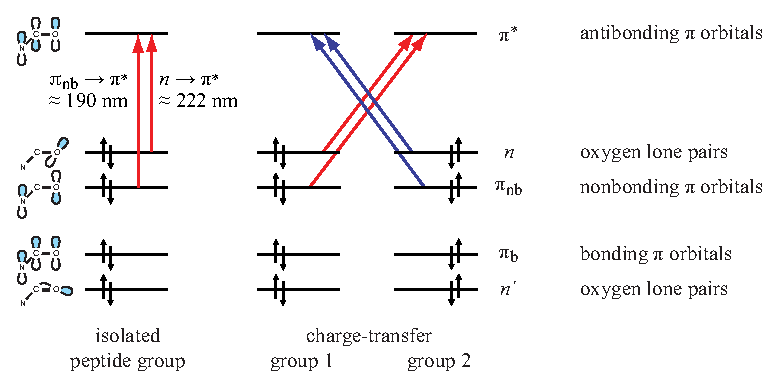
\includegraphics[width=12cm]{figures/amide-transitions.eps}
\caption{Parametrized transition for the peptide group (left) and charge-transfer between two neighboring peptide groups (right).}
\label{Fig:AmideTransitions}
\end{figure}

\label{Page:CT-parameters}

The charge-transfer chromophores (\verb'-CT......-') each consist of two peptide groups, parametrizing the CT between them. There are 19 CT parameter sets with different conformations (different $\phi$/$\psi$ angles between the monomers).\cite{Oakley:06:12414, Oakley:06:340, Bulheller:08:1866} The first four transitions are four local transitions, two for each monomer:

$n_1 \rightarrow \pi^*_1$, \hspace{3em}
$n_2 \rightarrow \pi^*_2$, \hspace{3em}
$\pi_{nb1} \rightarrow \pi^*_1$ \hspace{3em} \& \hspace{3em}
$\pi_{nb2} \rightarrow \pi^*_2$.

Transitions 5--8 are the actual charge-transfer transitions. They are also excitations from the $n$ and $\pi$ (nonbonding) orbital, but into the $\pi^*$ orbital of the neighboring peptide group (Figure~\ref{Fig:AmideTransitions}). In the parameter sets, they are not necessarily in the following order!

$n_1 \rightarrow \pi^*_2$, \hspace{3em}
$n_2 \rightarrow \pi^*_1$, \hspace{3em}
$\pi_{nb1} \rightarrow \pi^*_2$ \hspace{3em} \& \hspace{3em}
$\pi_{nb2} \rightarrow \pi^*_1$.

Table~\ref{Tab:CT-Chromophores} lists the data of the charge-transfer chromophores. These are required to identify a transition in the parameter set because the order of the transitions is not equal in all sets. By comparing the transition energies given in Table~\ref{Tab:CT-Chromophores} the sequence in the set can be easily determined. Very often, there are already comments in the parameter set, for example
\begin{verbatim}
     64          61659.    # 162.2 nm, Energy 1->6, n2 => Pi*1
\end{verbatim}
but if this is not the case, Table~\ref{Tab:CT-Chromophores} is required.

\begin{figure}
\enlargethispage{3em}
\centering
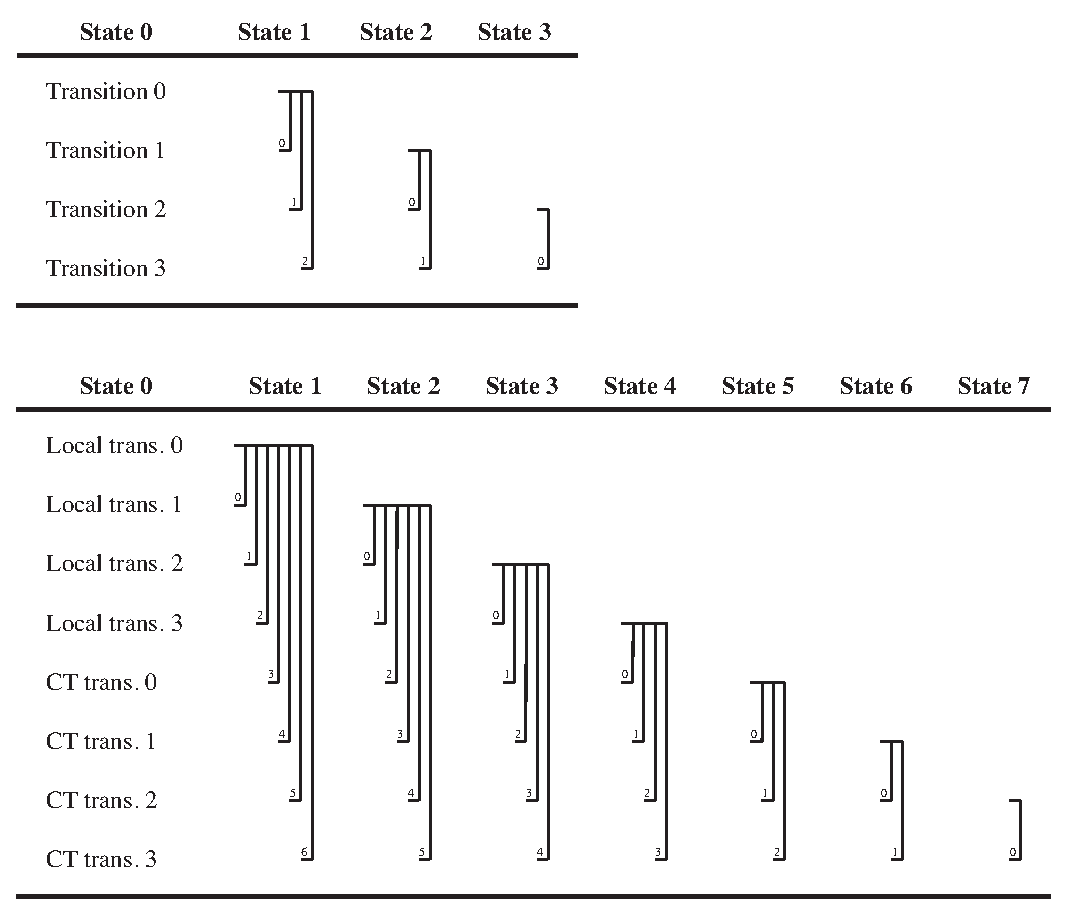
\includegraphics[width=0.9\textwidth]{figures/Parameter-set-transitions.eps}
\caption{Order of transitions in the states present in a parameter set for a standard chromophore with four transitions (top) and a charge-transfer chromophore (bottom). State 0 contains excitation from the ground state, higher states the interactions between transitions as depicted by the brackets.}
\label{Fig:ParameterSetStates}
\end{figure}

\begin{sidewaystable}
\captionsetup{width=0.8\textwidth, labelformat=simple, labelsep=colon}
\setlength{\tabcolsep}{1em}
\linespread{1.1}\normalsize
\centering

\begin{tabular}{cccccc}
\toprule
\textbf{Parameter set}     &
\textbf{Chromophore}       &
\textbf{Transition}        &
\textbf{Excitation/State}  &
\textbf{Wavelength} / nm   &
\textbf{Energy} / cm$^{-1}$ \\ \midrule

\multirow{4}{*}{NMA4FIT2~~\cite{Besley:99:9636}}  & \multirow{4}{*}{peptide bond}
		&   0   &   $n\rightarrow\pi^*$         &   220.0  &   45455   \\
	&	&   1   &   $\pi\rightarrow\pi^*$       &   193.0  &   51813   \\
	&	&   2   &   $\pi_{b}\rightarrow\pi^*$   &   129.4  &   77263   \\
	&	&   3   &   $n^\prime\rightarrow\pi^*$  &   122.6  &   81537   \\ \hline
  
\multirow{2}{*}{NMA99WDY~~\cite{Woody:99:2844}}   & \multirow{2}{*}{peptide bond}
		&   0   &   $n\rightarrow\pi^*$         &   220.0  &   45455   \\
	&	&   1   &   $\pi\rightarrow\pi^*$       &   190.0  &   52632   \\ \hline

\multirow{4}{*}{PHECASI3~~\cite{Rogers:03:11191}}  & \multirow{4}{*}{phenylalanine}
		&   0   &           $^1$L$_b$           &   263.1   &   38005   \\
	&	&   1   &           $^1$L$_a$           &   208.5   &   47953   \\
	&	&   2   &           $^1$B$_a$           &   191.1   &   52322   \\
	&	&   3   &           $^1$B$_b$           &   190.4   &   52532   \\ \hline
  
\multirow{4}{*}{TYRCASY4~~\cite{Rogers:03:11191}}  & \multirow{4}{*}{tyrosine}
		&   0   &           $^1$L$_b$           &   274.0   &   36492   \\
	&	&   1   &           $^1$L$_a$           &   216.4   &   46205   \\
	&	&   2   &           $^1$B$_a$           &   196.3   &   50932   \\
	&	&   3   &           $^1$B$_b$           &   192.4   &   51963   \\ \hline
  
\multirow{4}{*}{TRPCASH1~~\cite{Rogers:03:11191}}  & \multirow{4}{*}{tryptophan}
		&   0   &           $^1$L$_b$           &   282.5   &   35396   \\
	&	&   1   &           $^1$L$_a$           &   262.8   &   38053   \\
	&	&   2   &           $^1$B$_b$           &   204.3   &   48951   \\
	&	&   3   &           $^1$B$_a$           &   196.0   &   51032   \\ \hline
  
\multirow{4}{*}{ASNHIRST} & \multirow{4}{*}{arginine}
		&   0   &   $n\rightarrow\pi^*$         &    220.0  &   45455   \\
	&	&   1   &   $\pi\rightarrow\pi^*$       &    193.0  &   51813   \\
	&	&   2   &   $\pi_{b}\rightarrow\pi^*$   &    129.4  &   77263   \\
	&	&   3   &   $n^\prime\rightarrow\pi^*$  &    122.6  &   81537   \\ \hline
  
\multirow{4}{*}{GLNHIRST} & \multirow{4}{*}{glutamine}
		&   0   &   $n\rightarrow\pi^*$         &    220.0  &   45455   \\
	&	&   1   &   $\pi\rightarrow\pi^*$       &    193.0  &   51813   \\
	&	&   2   &   $\pi_{b}\rightarrow\pi^*$   &    129.4  &   77263   \\
	&	&   3   &   $n^\prime\rightarrow\pi^*$  &    122.6  &   81537   \\
\bottomrule
\end{tabular}
\caption{Data of matrix method parameter sets for the peptide backbone and side chains.}
\label{Tab:ParameterSets}
\end{sidewaystable}

\begin{sidewaystable}
\captionsetup{width=0.8\textwidth, labelformat=simple, labelsep=colon}
\caption[Wavelengths and oscillator strengths of the CT chromophores]
        {Wavelengths and oscillator strengths ($f$) of the charge-transfer chromophores. A mirror image of each geometry was created additionally to construct parameters, for example, for the left-handed helical and sheet regions of the Ramachandran plot.\cite{Oakley:06:12414, Oakley:06:340, Bulheller:08:1866}}
\label{Tab:CT-Chromophores}
\vspace{1em}

\centering
\linespread{1.4}\normalsize
\setlength{\tabcolsep}{1.5em}

\begin{tabular}{cccccccccc} \toprule
$\Phi/^\circ$                                         &
$\Psi/^\circ$                                         &
\multicolumn{2}{c}{$n_1 \rightarrow \pi_2^*$}         &
\multicolumn{2}{c}{$n_2 \rightarrow \pi_1^*$}         &
\multicolumn{2}{c}{$\pi_{nb1} \rightarrow \pi_2^*$}   & 
\multicolumn{2}{c}{$\pi_{nb2} \rightarrow \pi_1^*$}   \\ \cline{3-4} \cline{5-6} \cline{7-8} \cline{9-10}
 & 
 & 
 $\lambda/nm$ & $f$ &
 $\lambda/nm$ & $f$ &
 $\lambda/nm$ & $f$ &
 $\lambda/nm$ & $f$ \\ \midrule
\multicolumn{10}{c}{\textbf{strand structures}} \\
$180$   &  $180$  &  155.0  &  0.000  &  132.6  &  0.042  &  171.0  &  0.040  &  131.8  &  0.042  \\
$-135$  &  $135$  &  154.0  &  0.001  &  133.5  &  0.045  &  174.4  &  0.168  &  122.9  &  0.006  \\
$-120$  &  $120$  &  155.7  &  0.009  &  135.2  &  0.111  &  173.6  &  0.202  &  126.4  &  0.008  \\ [1ex]
\multicolumn{10}{c}{\textbf{hybrid structures}} \\
$-120$  &  $180$  &  153.2  &  0.029  &  142.1  &  0.056  &  167.0  &  0.015  &  138.5  &  0.047  \\
$-120$  &   $60$  &  166.7  &  0.215  &  134.9  &  0.021  &  159.9  &  0.056  &  135.2  &  0.005  \\
$-60$   &  $180$  &  156.1  &  0.004  &  135.9  &  0.023  &  170.9  &  0.051  &  136.4  &  0.058  \\ [1ex]
\multicolumn{10}{c}{\textbf{helical structures}} \\
$-74$   &   $-4$  &  138.2  &  0.022  &  162.9  &  0.091  &  153.1  &  0.002  &  145.9  &  0.010  \\
$-62$   &  $-41$  &  163.5  &  0.121  &  159.2  &  0.068  &  155.3  &  0.011  &  156.1  &  0.042  \\
$-48$   &  $-57$  &  156.9  &  0.123  &  162.1  &  0.013  &  164.4  &  0.014  &  152.7  &  0.015  \\
$-60$   &  $-60$  &  170.7  &  0.162  &  154.5  &  0.051  &  163.1  &  0.020  &  145.1  &  0.013  \\ \bottomrule
\end{tabular}
\end{sidewaystable}



% ----------------------------------------------------------------------------------------------------


\subsection{Generating the Spectra}

\subsubsection{Adding Bandshapes}

For a CD spectrum, the script \verb'bandshape' reads the line spectrum (\verb'.cdl'), adds Gaussian band shapes and saves the band spectrum to \verb'.cd'. The plots of an example spectrum before and after the convolution are shown below. The bandwidth 12.5~nm was found to match the experimental spectra best and is used by default.\cite{Hirst:03:11813, Bulheller:07:2020} Apart from Gaussian band shapes (default), it can also use Lorentzian and approximate Lorentzian curves. The spectrum is then scaled by a factor which is the number of residues in the protein. If a PDB file with the same base name is found, the number is determined from it, otherwise the scaling factor can be given via the command line option \verb'-s'. This scaling factor is the value stated in the \verb'$CONFIGURATION' block of the input file.

Common problems are spectra containing negative wavelengths. This can happen if two residues overlap too much and the Coulomb interaction goes through the roof. There are a couple of cases in CD190\cite{Bulheller:07:2020} and after lots of attempts the affected residues have been found and removed but without major changes to the spectrum, so generally this problem can be ignored if it is only affecting two or three residues. If negative wavelengths are encountered, \verb'bandshape' stops processing the file and issues an error to check this. With the \verb'-force' option, the spectrum is created nevertheless and \verb'bandshape' issues a warning that negative wavelengths have been found and how many.

\includegraphics[width=\textwidth]{figures/CD-Convolution.eps}

An LD spectrum is generated from a \verb'.vec' file\index{.vec file}, which lists the polarization vectors ($x$, $y$ and $z$ direction of the electric transition dipole moment) at each wavelength, for example like this:

{\small
\begin{verbatim}
     220.624106765373568  -0.003161481316737   0.010501954693544   0.013719453780057
     220.598672652223826  -0.005832340820421   0.000287929023263  -0.040574242107183
     220.570380334759164  -0.004506393382331   0.015418699095573   0.006213239718095
     220.537504034016962  -0.007808463093552   0.000615882128750  -0.031612650742340
\end{verbatim}
}

In the first step, the absorbance line spectra are created by taking the wavelengths and the respective vector component to produce the files named \verb'.x.abl', \verb'.y.abl' and \verb'.z.abl' (left in the plot below). The line spectra are then convoluted to yield the absorbance spectra \verb'.x.ab', \verb'.y.ab' and \verb'.z.ab' (middle). $z$ is defined as the parallel direction with respect to the flow direction in a Couette flow cell and, therefore, $x$ and $y$ are perpendicular directions. The actual perpendicular absorbance is considered as a rotational average over $x$ and $y$:

\begin{equation*}
A_{||} = A_z \quad \quad \quad A_\perp = \frac{1}{2}( A_x + A_y )
\end{equation*}

Both the parallel and perpendicular absorbance spectra are created, \verb'.para.ab' (the same as \verb'.z.ab' but created for consistency) and \verb'.perp.ab'. From those spectra, the LD spectrum \verb'.ld' (right) is calculated using the chosen method (LD, dichroic ratio or reduced LD). 

\includegraphics[width=\textwidth]{figures/LD-Convolution.eps}

For the calculation of the LD, three different methods can be used. Plain $LD$ is the standard, however, the dichroic ratio, $DR$, is a common standard for linear dichroism measurements. The reduced LD, $LD^r$, is obtained by dividing by the absolute absorbance.
%
\begin{equation*}
  LD  \quad = \quad A_{\parallel} - A_{\perp}
      \quad = \quad \mu_z^2 - \frac{1}{2} (\mu_x^2 + \mu_y^2)
\end{equation*}

\begin{equation*}
   LD^r \quad = \quad \frac{A_{\parallel} - A_{\perp}}{A} 
        \quad = \quad \frac{\mu_z^2 - \frac{1}{2} (\mu_x^2 + \mu_y^2)}
                {\frac{1}{3} ( \mu_x^2 + \mu_y^2 + \mu_z^2 ) }
\end{equation*}

\begin{equation*}
   DR   \quad = \quad \frac{A_{\parallel} - A_{\perp}}{A_{\parallel} + A_{\perp}}
        \quad = \quad \frac{\mu_z^2 - \frac{1}{2} (\mu_x^2 + \mu_y^2)}
                 {\mu_z^2 + \frac{1}{2} (\mu_x^2 + \mu_y^2)}
\end{equation*}

For consistency, \verb'bandshape' can also handle \verb'.abl' files and convolutes them to create the respective \verb'.ab' spectrum. However, the LD spectrum can only be calculated from the \verb'.vec' file and not from the single absorbance line spectra.

\begin{figure}[t]
\centering
\includegraphics[width=0.85\textwidth]{figures/Convolution-Diagrams.eps}
\caption{Workflow to create CD, absorbance and LD spectra.}
\label{Fig:CDandLD}
\end{figure}

If the \verb'PrintPol' parameter is set true when constructing the object (or the \verb'-pol' option given via the command line), DichroCalc also creates the \verb'.pol' file. This contains much more information than the \verb'.vec', for example, the polarizations for each single transition type, including the polarization tensors. The algorithm to calculate the LD has been developed for the two default transitions of peptides. Although it has now been extended to ``accept'' more than two transitions, this should be used with care and possibly checked for validity. The information in the \verb'.pol' file is for sure invalid if charge-transfer chromophores or side chains are included because the groups contain different transition sequences and types. If only peptide bonds are considered, the first transition is always $n\rightarrow\pi^*$, the second always $\pi\rightarrow\pi^*$ and it makes sense to calculate the polarization contributions for all first and all second transitions. However, in charge-transfer and side-chain chromophores the transitions are of a completely different kind.

\enlargethispage{1em}

Figure~\ref{Fig:CDandLD} shows the steps taken to create a CD and an LD spectrum, respectively, starting with the line spectrum files. 


% ----------------------------------------------------------------------------------------------------


\subsubsection{Plotting}

The \verb'plotspectrum' script is technically a front-end for gnuplot and produces an input file for the latter based on the given command line parameters. It is possible to write out the gnuplot command file as starting point and alter it to suit special needs. All parameters necessary to configure the plot can be given via the command line and the script can also be told to produce a bash script with the used options so that the style of the plot can be changed later or the command line itself be re-used. Due to the vast amount of options for the script, there is an extensive manual for it. In the following, only some particularities for using gnuplot for 3D graphs are covered.

2D spectra are produced by default and, therefore, an absorption spectrum does not require special parameters. Usually the $x$- and $y$ range are defined a bit different from the ranges chosen by gnuplot:

\begin{verbatim}
plotspectrum sig-abs  -x 42000 60000   -y 0 10000 
\end{verbatim}

Internally, the \verb'plot' command of gnuplot is used to produce the spectrum. To plot 3D, gnuplot needs to use the \verb'splot' command and this can be triggered by giving the identically named option to the script. Since the output files of Spectron contain many columns of which only a few are to be plotted, gnuplot has to be instructed so. The \verb'-using 4:3:5' option uses columns 4, 3, and 5 for $x$-, $y$-, and $z$-axis. For 3D plots that show surfaces, a PM3D color map improves the clarity of the plot, particularly if a 3D spectrum is viewed down the $z$-axis. A color surface map can be enabled with the option \verb'-pm3d'.

To be able to generate a PM3D surface, gnuplot requires grid data, that is the input data has to be divided into blocks with the same number of lines and in which one of the three coordinates is constant (whether this is $x$, $y$, or $z$ does not matter). This can be done by \verb'plotspectrum' with the \verb'grid' option. In the following examples, the third column is used to create valid gnuplot grid data:

\begin{verbatim}
plotspectrum sig-kI   -x -41900 -59900 -y 41900 59900 \
                      -using 4:3:5 -pm3d -contour 10 -grid 3 -splot

plotspectrum sig-kI   -x -41900 -59900 -y 41900 59900 \
                      -using 4:3:6 -pm3d -contour 10 -grid 3 -splot
\end{verbatim}



% ====================================================================================================


\newpage

\section{Course of a Calculation}

The routines are executed in a linear fashion during a calculation. At first the input file and matrix method parameters are parsed and the latter fitted to the chromophore coordinates of the protein. With the monopoles and dipole moments in place the Hamiltonian matrix is constructed, diagonalized, and the eigenvalues and eigenvectors used to calculate the dipole moments of the interacting system. These allow the actual dichroism calculation and the line spectrum is printed as result. The following explains the working of DichroCalc in detail.


% ----------------------------------------------------------------------------------------------------


\subsection{Initializing the Object}
\label{Sec:InitializeingTheObject}

A program using the \verb'Dichro::' class only needs to include the \verb'dichrocalc.h' header file (apart from being linked with the \verb'libdichrocalc.a' library). The prototype of the object is

\begin{verbatim}
Dichro::Dichro ( string InFile, string Params, bool Verbose, int Debug,
                 bool PrintVec, bool PrintPol, bool PrintMat )
\end{verbatim}

The following parameters may or have to be given to the constructor. Only the input file is mandatory, all other parameters are optional.

\begin{itemize}
\item \verb'InFile' (mandatory) \\
The input file (\verb'inp') with information on the system.

\item \verb'Params' \\
A directory with the files containing the parameter sets. The filenames have to be identical with the individual names given in the input file and a \verb'.par' extension. Only the parameter sets specified in the input file will actually be read in. If this parameter is omitted then \verb'~/bin/params' is used. The default folder can be changed in the constructor.

\item \verb'Verbose' \\
If true, this instructs DichroCalc to output information along the way.

\item \verb'Debug' \\
An integer value between 0 and 5. If greater than 0, DichroCalc writes debug information such as the read input data and intermediate results to the \verb'.dbg' file. The higher this value, the more information is printed. For values 4 and 5, in addition to the debug file the \verb'.fit' file is created with information on the parameter fitting.

\item \verb'PrintVec' \\
Creates the \verb'.vec' file containing the polarization vectors for each transition. The script \verb'bandshape' uses this file to calculate the absorption and LD spectra.

\item \verb'PrintPol' \\
Creates the \verb'.pol' file with the polarizations broken down into the contributions of the single transitions.

\item \verb'PrintMat' \\
Creates the \verb'.mat' file containing the Hamiltonian matrix, eigenvectors, and eigenvalues.

\end{itemize}

\newpage

The constructor directly performs the calculation, the results can be retrieved from the object right after creating it. A minimum program using the library may look like this:

\begin{verbatim}
<-- standard header files -->

#include "dichrocalc.h"

int main ( void )
{
   Dichro *DichroCalc;
   DichroCalc = new Dichro ( "file.inp",  "parameters/" );

   cout << setw(15) << DichroCalc->DC_Results.Hamiltonian << "\n\n";
   cout << setw(15) << DichroCalc->DC_Results.Eigenvectors << "\n\n";
   cout << setw(15) << DichroCalc->DC_Results.Eigenvalues << "\n\n";
   
   return 0;
}
\end{verbatim}

The course of the calculation is laid out in the constructor in \verb'readinput.cpp'.


% ----------------------------------------------------------------------------------------------------


\subsection{Reading the Input (\texttt{readinput.cpp})}

\paragraph{The Input File:}
The function \verb'ReadInput' parses the \verb'.inp' file and fills the information into the \verb'DC_Input' structure (Sec.~\ref{Sec:DC_Input}). The file is extension is added if it was omitted. Possible errors may be unknown options in the \verb'$CONFIGURATION' section, or more or less than the expected number of columns in any of the other blocks.

A general syntax check of the input is performed by \texttt{CheckInputData}. This includes tests whether the chromophore types used in the \texttt{\$CHROMOPHORES} block are actually defined under \texttt{\$PARAMETERS} and if all atoms used for the chromophores are present under \texttt{\$COORDINATES}.

\paragraph{The parameter sets:}
If no errors have been found, the parameter sets defined in the input file are read by \verb'ReadParameters'. The function creates a separate structure for each set and collects these in the vector \verb'DC_ParSets' (Sec.~\ref{Sec:DC_ParSets}). The sets are read in the same sequence as given in the input file and the index in the \verb'DC_ParSets' vector is, therefore, the index used under \verb'CHROMOPHORES' to assign the parameters to the groups in the protein. Every parameter set is read in completely, regardless of the number of transitions considered according to the input file. This was implemented like this to keep the parsing routine as general as possible.

After reading the atoms, a reference vector for the chromophore is calculated. This is a calculation similar to the center of mass determination, adding up the coordinates of all atoms (taking their individual weighting factors into account). This position vector is required for the fitting of the parameters to the chromophores.


% ----------------------------------------------------------------------------------------------------


\subsection{Fitting the Parameters (\texttt{fitparameters.cpp})}

In \verb'FitParameters', for each chromophores defined in the \verb'$CHROMOPHORES' section a copy of the respective parameter set a created and its dipole moments and monopoles moved to the position of the chromophore. A Singular Value Decomposition routine (SVD) is used to fit the parameters. If the debug option is greater than 4, all intermediate steps of the fitting process are printed to the \verb'.fit' file.

As preparation for the SVD, two matrices are created from the parameter set atoms and the PDB atoms, with the $x$,$y$,$z$ coordinates as columns. The parameter set atoms are located at the origin in the first place. In order to perform the SVD, the atoms of the chromophore are moved to the origin as well and, therefore, a position vector is determined for the group and subtracted from each atom. The two matrices are the input for the SVD that is performed by the function \verb'RotationMatrix'. A rotation matrix is determined that leads to the best fit when it is applied to parameter set coordinates such as the dipole moments and monopoles. The atoms and monopoles are moved to the original position by adding the position vector after rotation.

For a Matrix $M$, an SVD is defined as
\begin{equation*}
M = U \cdot W \cdot V^T \quad .
\end{equation*}

The matrices $U$, $W$, and $V$ are determined for the matrix of the parameter set atoms. $W$ is a diagonal matrix, its elements are the singular values. The inverse of $W$, $W^I$, is calculated by taking the reciprocals of all elements. If the system is planar the $W$ matrix of the decomposition shows a 0 in one column and the calculation the reciprocal values would, therefore, lead to a division by zero. If this is encountered, an additional point off the plane is added to both matrices by calculating the cross product of the vectors between the first three atoms. With $W^I$, the pseudo inverse of the parameter set matrix, $P_p$, can then be calculated as
\begin{equation*}
P_p = V \cdot W^I \cdot U^T \quad ,
\end{equation*}
and it follows the non-unitary rotation matrix, $R$ for the matrix of the chromophore group atoms, $M_g$:
\begin{equation*}
R = M_g \cdot P_p^T \quad .
\end{equation*}
 
A rotation with the non-unitary matrix allows some stretching of the rotated system and this changes the monopole distances and dipole moment lengths (calculations showed a slight worsening of the spectra). Therefore, the determination of the unitary rotation matrix is crucial. A second SVD is performed for the non-unitary rotation matrix, $R$:
\begin{equation*}
R = U \cdot W \cdot V^T \quad
\end{equation*}
and the unitary rotation matrix, $R^{uni}$, calculated using
\begin{equation*}
R^{uni} = U \cdot V^T
\end{equation*}

It is in this routine where the transitions to use in the calculations are selected from the fully parsed parameter set. That is, if two transitions are requested for the \verb'NMA4FIT2' set of the peptide bond in the input file, \verb'FitParameters' will only fit the first two of the available four transitions.

In the \verb'ReadParameters'-function, the parameter set is read in with the transitions divided up into states. The excitations from the ground state are combined in state \verb'0', and interactions between states are combined in higher states (Fig.~\ref{Fig:ParameterSetStates}, page~\pageref{Fig:ParameterSetStates}). The last state contains the permanent moments. The division into separate states would be cumbersome during the interaction calculation and, therefore, the required transitions including the ones in higher states are added one after another to the \verb'DC_System.Trans' vector. Only permanent moments are stored separately in \verb'DC_System.Perm'. To keep track of the origin of the transitions in the \verb'DC_System.Trans' vector, the variable \verb'Origin' stores the parameter set, state and transition it is originating from. This is printed to the debug file, for example:
\begin{verbatim}
   Transition 4 (Group 0)
   
      Parameter set:   NMA4FIT2 - State 1 - Transition 0
\end{verbatim}

This shows that the 5$^{th}$ transition of the first group is the first transition, taken from the second state of the \verb'NMA4FIT2' parameter set.

% ----------------------------------------------------------------------------------------------------


\subsection{Setting up the Hamiltonian Matrix (\texttt{matrix.cpp})}

The order of the states along the diagonal is exactly as given in the input file. First all transitions of group 0, then all transitions of group 1, and so on and so forth. Mind that the groups are sorted by parameter set type, that is first peptide groups, then charge-transfer groups, and the side chains. This means that the peptide bond, side chain group and charge-transfer contribution of a tyrosine residue will end up separated in the matrix, even though the transitions are localized on the same group. This has no influence on the result.

For example, for a dipeptide and two transitions per group, the important sections in the input file would be
\begin{verbatim}
$PARAMETERS
#   name      trans.   #   type
    NMA4FIT2    2      #    1
$END

$CHROMOPHORES
#  type    atoms
    1          3       4       5
    1          7       8       9
$END
\end{verbatim}

The Hamiltonian matrix constructed for these groups has the form\cite{Bulheller:07:2020}
%
\begin{equation}
	\hat{H} =
	\left(
		\begin{array}{cccc}
			E_{1n\pi^*}                        &  \colblue{V_{1n\pi^*;\; 1\pi\pi^*}} &  \colred{V_{1n\pi^*;\; 2n\pi^*}}   & \colred{V_{1n\pi^*;\; 2\pi\pi^*}}   \\
			\colblue{V_{1n\pi^*;\; 1\pi\pi^*}} &  E_{1\pi\pi^*}                      &  \colred{V_{1n\pi^*;\; 2\pi\pi^*}} & \colred{V_{1\pi\pi^*;\; 2\pi\pi^*}} \\
			\colred{V_{1n\pi^*;\; 2n\pi^*}}    & \colred{V_{1\pi\pi^*;\; 2n\pi^*}}   &  E_{2n\pi^*}                       & \colblue{V_{2n\pi^*;\; 2\pi\pi^*}}  \\
			\colred{V_{1n\pi^*;\; 2\pi\pi^*}}  & \colred{V_{1\pi\pi^*;\; 2\pi\pi^*}} & \colblue{V_{2n\pi^*;\; 2\pi\pi^*}} & E_{2\pi\pi^*}                       \\
		\end{array}
	\right) \;.
	\label{Eqn:HamiltonianMatrix}
\end{equation}
%
\colblue{$V_{ii}$} are interactions between states on the same group and \colred{$V_{ij}$} are interactions between different groups, respectively. Interactions are determined by calculating the Coulomb-Coulomb interactions of all monopoles of the involved transitions. For interactions on \colred{different groups} these are only the respective ground state excitations, for example, the $\pi\rightarrow\pi^*$ transitions on groups 0 and 1. For interactions on the \colblue{same group} this is the transition of the respective group with the permanent moments on \emph{all} other groups.

If two groups are too close due to a bad fitting of the parameters or a wrong PDB structure, the calculation of the interaction leads to a Coulomb-explosion. This is evident by abnormally-large matrix elements and very high or negative wavelengths. For each group overlap there is usually one or two negative wavelengths at the beginning and the same number of large wavelengths at the end of the line spectrum file (\verb'.cdl'). The \verb'bandshape' script will flag this up and not create the spectrum in this case. However, it was found that it usually does not affect the spectrum much. If there only a few ``bad'' transitions, the creation of the band spectrum can be forced using the \verb'-force' option.

The problem of overlapping monopole charges also means that the interactions of two charge-transfer groups sharing one monomer have to be ignored. To catch such cases, all atoms of both groups are compared to check, whether any are shared between the chromophores. The Hamiltonian for a tripeptide, showing only one charge-transfer transition per peptide group for clarity, has the form\cite{Bulheller}

\begin{equation}
\linespread{1.3}\normalsize
	\hat{H} =
	\left(
		\begin{array}{ccccc}
			E_{Local_1}    & V_{E_1;\; E_2} & V_{E_1;\; E_3} & \colgreen{V_{E_1;\; CT_{12}}} & \colgreen{V_{E_1;\; CT_{23}}} \\
			V_{E_1;\; E_2} & E_{Local_2}    & V_{E_2;\; E_3} & \colgreen{V_{E_2;\; CT_{12}}} & \colgreen{V_{E_2;\; CT_{23}}} \\
			V_{E_1;\; E_3} & V_{E_2;\; E_3} & E_{Local_3}    & \colgreen{V_{E_3;\; CT_{12}}} & \colgreen{V_{E_3;\; CT_{23}}} \\
			\colgreen{V_{E_1;\; CT_{12}}} &  \colgreen{V_{E_2;\; CT_{12}}} & \colgreen{V_{E_3;\; CT_{12}}} & \colgreen{CT_{12}} & \colgreen{0}       \\
			\colgreen{V_{E_1;\; CT_{23}}} &  \colgreen{V_{E_2;\; CT_{23}}} & \colgreen{V_{E_3;\; CT_{23}}} & \colgreen{0}       & \colgreen{CT_{23}} \\
		\end{array}
	\right) \;.
	\label{Eqn:CT-HamiltonianMatrix}
\end{equation}

Interactions involving charge-transfer groups are \colgreen{green}. The blocks involving solely local excitations are as defined in Equation~\ref{Eqn:HamiltonianMatrix}. The zeros in Equation~\ref{Eqn:CT-HamiltonianMatrix} reflect that charge-transfer chromophores sharing a common peptide group are not allowed to interact. In Equation~\ref{Eqn:CT-HamiltonianMatrix} the first charge-transfer chromophore consists of peptide groups one and two, whereas the latter spans groups two and three.

The matrix is then diagonalized using either the Jacobi or the Householder method, depending on which line of the two is commented. According to the NewMat documentation, the Jacobi method is extremely reliable but much slower than the Householder algorithm.

All results calculated in \verb'HamiltonianMatrix' and the following function, \verb'CD_Calculation', are collected in the data structure \verb'DC_Results' (see Sec.~\ref{Sec:DC_Results}, page~\pageref{Sec:DC_Results}). Notably, the results are accessible twice in the data structure, on a per-transition basis and per-group basis. The former is the way the algorithm works and the interactions are calculated, starting with the first transition of the first group in the first diagonal element. After the diagonalization, the data are copied for each group, including the respective submatrix.

If the object was constructed with the \verb'PrintMat' option then the Hamiltonian matrix, eigenvectors, and eigenvalues are printed to the \verb'.mat' file.


% ----------------------------------------------------------------------------------------------------

\pagebreak

\subsection{The Dichroism Calculation (\texttt{dichroism.cpp})}

In the function \verb'CD_Calculation', first of all the initial magnetic transition dipole moments are \emph{somehow} converted. This involves the electric transition dipole moments, transition energy and the magic number $3.3879\cdot10^{-6}$, whose origin has not yet been identified. In the following, the electric and transition dipole moments of the interacting system are calculated, involving the eigenvectors and eigenvalues.

The rotational strength is given by the Rosenfeld equation:
%
\begin{equation}
	R^{0k} = Im ( \langle \psi^0 | \vec{\mu} | \psi^k \rangle 
				\cdot
				\langle \psi^k | \vec{m} | \psi^0 \rangle) \;\textrm{,}
\label{Eqn:Rosenfeld}
\end{equation}
%
Therefore, the rotational strength is calculated by multiplying the coordinates of both dipole moments of the transitions. The dipole strength is calculated taking the square of the electric transition dipole moment.

The units of the matrix, eigenvectors and eigenvalues are wavenumbers. The eigenvalues are the transition energies of the interacting system, they are converted to nanometers and printed to the line spectrum file (\verb'.cdl') with the rotational strength being the $y$-value.


% ====================================================================================================


\newpage

\section{Object Structure and Variables}

\label{Sec:ObjectStructure}

All data read and produced by the program were highly capsulated in nested data structures. This was done in order to make the routines that read the input and parameter files as well as the produced data in general re-usable in other programs. In particular these structures are:

\begin{itemize}
\item \verb'DC_Input' \\
All data read from the input file (\verb'.inp', the extension may be omitted). Filled by the function \texttt{ReadInput} in \verb'readinput.cpp'.

\item \verb'DC_ParSets' \\
Data read from the parameter set files (\verb'.par'). Filled by the function \texttt{ReadParameters} in \verb'readinput.cpp'.

\item \verb'DC_System' \\
Combined information from the input and parameter files, that is the complete system with the parameter sets fitted to the protein chromophores. Created by function \texttt{FitParameters} in \verb'fitparameters.cpp'.

\item \verb'DC_Results' \\
Calculated results using only the data stored in \verb'DC_System'. Filled by several functions in \verb'matrix.cpp' and \verb'dichroism.cpp'.
\end{itemize}

The data structures are listed in detail in the following sections. The structures are created by nesting classes using vectors and sub-classes. For each user-defined class there is usually a dedicated output routine that prints it to the debug file. The parent class a particular branch in a tree diagram was created from is given \texttt{\textit{slanted monospaced}} next to the branch.


% ----------------------------------------------------------------------------------------------------


\newpage

\subsection{Input Data}
\label{Sec:DC_Input}

The data read from the input file (\verb'.inp') is collected in the following structure named after the respective section in the input.

\begin{tabular}{p{7.5cm}l}
\verb'DC_Input' \class{Input}                             &                                                                \\
\tab \textbar --- \verb'Configuration' \class{InputConfiguration} & data read from the \verb'$CONFIGURATION' block         \\
\tab \textbar \tab \textbar  --- \verb'BBTrans'           & --1 = all backbone trans., 0--3 = specific BB trans.           \\
\tab \textbar \tab \textbar  --- \verb'CTTrans'           & --1 = all CT transitions, 0--3 = specific CT  trans.           \\
\tab \textbar \tab \textbar  --- \verb'Factor'            & scale factor for intensities (number of residues)              \\
\tab \textbar \tab \textbar  --- \verb'MinWL'             & the minimum wavelength                                         \\
\tab \textbar \tab \Endangle --- \verb'MaxWL'             & the maximum wavelength                                         \\
% \tab \textbar \tab \textbar  --- \verb'Debug'             & 0 = no debug output, 1--5 = increasing output to \verb'.dbg'   \\
% \tab \textbar \tab \textbar  --- \verb'Verbose'           & verbose output during the calculation                          \\
% \tab \textbar \tab \Endangle --- \verb'Params'            & directory with the parameter files (\verb'.par')               \\
\tab \textbar                                             &                                                                \\
\tab \textbar --- \verb'Parameters' \class{InputParameters} & data read from the \verb'$PARAMETERS' block                  \\
\tab \textbar \tab \textbar  --- \verb'Name'              & names of the parameter sets (also filenames)                   \\
\tab \textbar \tab \textbar \tab \Endangle --- \atType    & \emph{string}                                                  \\
\tab \textbar \tab \Endangle --- \verb'Trans'             & number of transitions of the parameter sets                    \\
\tab \textbar \tab \tab \Endangle ---  \atType            & \emph{int}                                                     \\
\tab \textbar                                             &                                                                \\
\tab \textbar --- \verb'Chromophores' \class{InputChromophores}& data read from the \verb'$CHROMOPHORES' block             \\
\tab \textbar \tab \textbar  --- \verb'Type'              &                                                                \\
\tab \textbar \tab \textbar \tab \Endangle --- \atGroup   & \emph{int}, index in \verb'.Parameters' specifying the type    \\
\tab \textbar \tab \Endangle --- \verb'Atoms'             & the indices of the atoms in \verb'.Coordinates'                \\
\tab \textbar \tab \tab \Endangle --- \atGroup            &                                                                \\
\tab \textbar \tab \tab \tab \Endangle --- \atAtom        & \emph{int}                                                     \\
\tab \textbar                                             &                                                                \\
\tab \Endangle --- \verb'Coordinates' \class{InputCoordinates} & data read from the \verb'$COORDINATES' block              \\
\tab \tab \textbar --- \verb'Groups'                      & the $xyz$ coordinates of the atoms                             \\
\tab \tab \textbar \tab \Endangle --- \atGroup            &                                                                \\
\tab \tab \textbar \tab \tab \Endangle --- \atCoord       & \emph{double}                                                  \\
\tab \tab \textbar --- \verb'Atoms'                       & atom indices as given in \verb'.Chromophores'                  \\
\tab \tab \textbar \tab \Endangle --- \atGroup            & \emph{int}                                                     \\
\tab \tab \Endangle--- \verb'Labels'                      & the PDB atom labels (e.g.\ \verb'CA')                          \\
\tab \tab \tab \Endangle --- \atGroup                     & \emph{string}                                                  \\
\end{tabular}


\subsection*{Relevant Output Functions}

\begin{itemize}
\item \verb'void Dichro::OutputInputClass ( void )'
\item \verb'void Dichro::OutputInputConfigurationClass ( void )'
\item \verb'void Dichro::OutputInputParametersClass ( void )'
\item \verb'void Dichro::OutputInputChromophoresClass ( void )'
\item \verb'void Dichro::OutputInputCoordinatesClass ( void )'
\end{itemize}


% ----------------------------------------------------------------------------------------------------


\newpage

\subsection{Parameter Set Data}
\label{Sec:DC_ParSets}

For each chromophore (e.g.\ amide bond, charge-transfer group) a parameter set is read from a file (\verb'.par'). These files are stored in a directory that is given to the program via the \verb'-p/--params' option. All information read from the parameter set files is stored in the following structure.

\begin{tabular}{p{9.5cm}l}
\verb'DC_ParSets' \class{ParSet}                                           &                              \\
\tab \Endangle --- \atType \class{ParSet}                                  & \hspace{-3cm} (the index is the type in \verb'.Parameters') \\
\tab \tab \textbar --- \verb'Name'                                         & \hspace{-3cm} \emph{string}  \\
\tab \tab \textbar  --- \verb'NumberOfAtoms'                               & \hspace{-3cm} \emph{int}     \\
\tab \tab \textbar  --- \verb'NumberOfTransitions'                         & \hspace{-3cm} \emph{int}     \\
\tab \tab \textbar  --- \verb'ChargeTransfer'                              & \hspace{-3cm} \emph{bool}    \\
\tab \tab \textbar  --- \verb'Atoms'                                       & \hspace{-3cm}                \\
\tab \tab \textbar  \tab \Endangle --- \atAtom                             & \hspace{-3cm}                \\
\tab \tab \textbar  \tab \tab \textbar --- \verb'Label'                    & \hspace{-3cm} \emph{string}  \\
\tab \tab \textbar  \tab \tab \textbar  --- \verb'Weighting'               & \hspace{-3cm} \emph{double}  \\
\tab \tab \textbar  \tab \tab \Endangle --- \verb'Coord'.\atCoord          & \hspace{-3cm} \emph{double}  \\
\tab \tab \textbar  \tab                                                   & \hspace{-3cm}                \\
\tab \tab \textbar  \tab                                                   & \hspace{-3cm}                \\
\tab \tab \textbar  --- \verb'Reference.at(0,1,2)'                         & \hspace{-3cm} \emph{double}  \\
\tab \tab \textbar  \tab                                                   &                              \\
\tab \tab \Endangle --- \verb'States'                                      &                              \\
\tab \tab \tab \Endangle --- \atState                                      &                              \\
\tab \tab \tab \tab \Endangle --- \atTrans \class{ParSetTrans}             &                              \\
\tab \tab \tab \tab \tab \textbar  --- \verb'Permanent'                    & \emph{bool}                  \\
\tab \tab \tab \tab \tab \textbar  --- \verb'Energy'                       & \emph{double} (cm$^{-1}$)    \\
\tab \tab \tab \tab \tab \textbar  --- \verb'Wavelength'                   & \emph{double} (nm)           \\
\tab \tab \tab \tab \tab \textbar  --- \verb'ScaleFactor'                  & \emph{double}                \\
\tab \tab \tab \tab \tab \textbar  --- \verb'EDM.'\atCoord                 & \emph{double}                \\
\tab \tab \tab \tab \tab \textbar  --- \verb'MDM.'\atCoord                 & \emph{double}                \\
\tab \tab \tab \tab \tab \textbar  --- \verb'NumberOfMonopoles'            & \emph{int}                   \\
\tab \tab \tab \tab \tab \Endangle --- \verb'Monopoles'                    &                              \\
\tab \tab \tab \tab \tab \tab \Endangle --- \atMono \class{ParSetMonopole} &                              \\
\tab \tab \tab \tab \tab \tab \tab \textbar  --- \verb'Charge'             & \emph{double}                \\
\tab \tab \tab \tab \tab \tab \tab \Endangle --- \verb'Coord.'\atCoord     & \emph{double}                \\
\end{tabular}


\subsection*{Relevant Output Functions}

\begin{itemize}
\item \verb'void Dichro::OutputParSetClass ( ParSet* )'
\item \verb'void Dichro::OutputParSetTransClass ( ParSetTrans*, int )' \\
      (the \verb'int'eger is an optional number of the transition)
\item \verb'void Dichro::OutputParSetMonopoleClass ( ParSetMonopole* )'
\end{itemize}


% ----------------------------------------------------------------------------------------------------


\newpage

\subsection{Processed and Calculated Data}
\label{Sec:DC_System}

\begin{tabular}{p{10.0cm}l}
\verb'DC_System' \class{System}                      & \hspace{-8em} all information necessary to describe the system  \\
\tab \textbar  --- \verb'NumberOfAtoms'              & \hspace{-8em} \emph{int}, number of atoms in all parameter sets \\
\tab \textbar  --- \verb'NumberOfGroups'             & \hspace{-8em} \emph{int}, number of chromophores                \\
\tab \textbar  --- \verb'NumberOfTransitions'        & \hspace{-8em} \emph{int}, combined number of transitions        \\
\tab \textbar  --- \verb'MatrixDimension'            & \hspace{-8em} \emph{int}, same as number of transitions         \\
\tab \textbar                                        &                                                                 \\
\tab \textbar  --- \verb'Atoms'                      &                                                                 \\
\tab \textbar \tab \Endangle  --- \atAtom            &                                                                 \\
\tab \textbar \tab \tab \Endangle --- \atCoord       & \emph{double}                                                   \\
\tab \textbar                                        &                                                                 \\
\tab \Endangle --- \verb'Groups'                                               &                                       \\
\tab \tab \Endangle --- \atGroup \class{SystemGroup}                           &                                       \\
\tab \tab \tab \textbar  --- \verb'Atoms'                                      &                                       \\
\tab \tab \tab \textbar \tab \Endangle --- \atAtom                             &                                       \\
\tab \tab \tab \textbar \tab \tab \Endangle --- \atCoord                       & \emph{double}                         \\
\tab \tab \tab \textbar  --- \verb'AtomIndices'                                &                                       \\
\tab \tab \tab \textbar \tab \Endangle --- \atAtom                             &                                       \\
\tab \tab \tab \textbar \tab \tab \Endangle --- \atIndex                       & \emph{int}                            \\
\tab \tab \tab \textbar  --- \verb'Reference'                                  &                                       \\
\tab \tab \tab \textbar \tab \Endangle --- \atCoord                            & \emph{double}, the reference vector   \\
\tab \tab \tab \textbar  --- \verb'NumberOfTransitions'                        &                                       \\
\tab \tab \tab \textbar  --- \verb'ParameterSet'                               & \emph{string}                         \\
\tab \tab \tab \textbar  --- \verb'Trans'                                      &                                       \\
\tab \tab \tab \textbar \tab \Endangle --- \atTrans \class{SystemTransition}   &                                       \\
\tab \tab \tab \textbar \tab \tab \textbar  --- \verb'Origin'                  & \emph{string} (parameter set, state \& trans.) \\
\tab \tab \tab \textbar \tab \tab \textbar  --- \verb'Permanent'               & \emph{bool}                           \\
\tab \tab \tab \textbar \tab \tab \textbar  --- \verb'Energy'                  & \emph{double} (in cm$^{-1}$)          \\
\tab \tab \tab \textbar \tab \tab \textbar  --- \verb'Wavelength'              & \emph{double} (in nm)                 \\
\tab \tab \tab \textbar \tab \tab \textbar  --- \verb'NumberOfMonopoles'       & \emph{int}                            \\
\tab \tab \tab \textbar \tab \tab \textbar  --- \verb'Monopoles'               &                                       \\
\tab \tab \tab \textbar \tab \tab \textbar  \tab \Endangle --- \atMono \class{ParSetMonopole} &                        \\
\tab \tab \tab \textbar \tab \tab \textbar  \tab \tab \textbar  --- \verb'Charge'         & \emph{double}              \\
\tab \tab \tab \textbar \tab \tab \textbar  \tab \tab \Endangle --- \verb'Coord.'\atCoord & \emph{double}              \\
\tab \tab \tab \textbar \tab \tab \textbar  \tab                               &                                       \\
\tab \tab \tab \textbar \tab \tab \textbar  --- \verb'EDM'                     & electric trans. dipole moment         \\
\tab \tab \tab \textbar \tab \tab \textbar  \tab \Endangle --- \atCoord        & \emph{double}                         \\
\tab \tab \tab \textbar \tab \tab \textbar                                     &                                       \\
\tab \tab \tab \textbar \tab \tab \Endangle --- \verb'MDM'                     & magnetic trans. dipole moment         \\
\tab \tab \tab \textbar \tab \tab \tab \Endangle --- \atCoord                  & \emph{double}                         \\
\tab \tab \tab \Endangle --- \verb'Perm'                                       &                                       \\
\tab \tab \tab \tab \Endangle --- \atPerm  \class{SystemTransition}            & the permanent moments                 \\
\tab \tab \tab \tab \tab\dotbar\hspace{0.5em}---\emph{same structure as Trans} &                                       \\
\end{tabular}

\vspace{1em}

\newpage

\verb'DC_System.NumberOfTransitions' is the sum of transitions on all chromophores. This counts only actual transitions, from the ground state to the excited state (e.g.\ $n\rightarrow\pi^*$ and $\pi\rightarrow\pi^*$), but not higher excitations. It is the same number as \verb'DC_System.MatrixDimension', it is just stored twice to make some commands in the code easier to read/interpret.

\verb'DC_System.Groups.'\atGroup\verb'.'\atTrans.\verb'NumberOfTransitions' is determined the same way and holds the number of ground-to-excited state transitions for a particular group.


\subsection*{Relevant Output Functions}

\begin{itemize}
\item \verb'void Dichro::OutputSystemClass ( void )'
\item \verb'void Dichro::OutputSystemGroupClass ( SystemGroup*, int )' \\
      (the \verb'int'eger is an optional number of the group)
\item \verb'void Dichro::OutputSystemTransitionClass ( SystemTransition*, int )' \\
      (the \verb'int'eger is an optional number of the transition)
\end{itemize}


% ----------------------------------------------------------------------------------------------------


\newpage

\subsection{Results}
\label{Sec:DC_Results}

\begin{tabular}{p{8.5cm}l}
\verb'DC_Results' \class{Results}                          & all information calculated from \verb'DC_System'  \\
\tab \textbar  --- \verb'NumberOfAtoms'                    & \emph{int}, number of atoms in all parameter sets \\
\tab \textbar  --- \verb'NumberOfGroups'                   & \emph{int}, number of chromophores                \\
\tab \textbar  --- \verb'NumberOfTransitions'              & \emph{int}, combined number of transitions        \\
\tab \textbar  --- \verb'MatrixDimension'                  & \emph{int}, same as number of transitions         \\
\tab \textbar  --- \verb'Hamiltonian.element(row,col)'     & \emph{SymmetricMatrix}                            \\
\tab \textbar  --- \verb'Eigenvectors.element(row,col)'    & \emph{Matrix}                                     \\
\tab \textbar  --- \verb'Eigenvalues.element(row,row)'     & \emph{DiagonalMatrix}                             \\
\tab \textbar                                              &                                                   \\
\tab \textbar  --- \verb'Groups'                           &                                                   \\
\tab \textbar \tab \Endangle --- \atGroup \class{ResultsGroup}                & access via the group                \\
\tab \textbar \tab \tab \textbar  --- \verb'NumberOfTransitions'              & \emph{int}                          \\
\tab \textbar \tab \tab \textbar  --- \verb'ChargeTransfer'                   & \emph{bool}                         \\
\tab \textbar \tab \tab \textbar  --- \verb'ParameterSet'                     & \emph{string}                       \\
\tab \textbar \tab \tab \textbar  --- \verb'Energy'.\atTrans                  & \emph{double} (in cm$^{-1}$)        \\
\tab \textbar \tab \tab \textbar  --- \verb'Wavelength'.\atTrans              & \emph{double} (in nm)               \\
\tab \textbar \tab \tab \textbar  --- \verb'DipoleStrength'.\atTrans          & \emph{double}                       \\
\tab \textbar \tab \tab \textbar  --- \verb'RotationalStrength'.\atTrans      & \emph{double}                       \\
\tab \textbar \tab \tab \textbar  --- \verb'OscillatorStrength'.\atTrans      & \emph{double}                       \\
\tab \textbar \tab \tab \textbar  --- \verb'Submatrix.element(row,col)'       & \emph{SymmetricMatrix}              \\
\tab \textbar \tab \tab \textbar                                              &                                     \\
\tab \textbar \tab \tab \textbar  --- \verb'Reference'.\atTrans               & Reference vectors of the groups     \\
\tab \textbar \tab \tab \textbar  \tab \hspace{1.8cm} \Endangle --- \atCoord  & \emph{double}                       \\
\tab \textbar \tab \tab \textbar  --- \verb'EDM'.\atTrans                     & Electric transition dipole moments  \\
\tab \textbar \tab \tab \textbar  \tab \tab \Endangle --- \atCoord            & \emph{double}                       \\
\tab \textbar \tab \tab \textbar  --- \verb'MDM'.\atTrans                     & Magnetic transition dipole moments  \\
\tab \textbar \tab \tab \textbar  \tab \tab \Endangle --- \atCoord            & \emph{double}                       \\
\tab \textbar \tab \tab \Endangle --- \verb'PolarizationVector'.\atTrans      & Polarization vectors                \\
\tab \textbar \tab \tab \tab \tab \tab \tab \tab \Endangle --- \atCoord       & \emph{double}                       \\
\tab \textbar                                                                 &                                     \\
\tab \Endangle --- \verb'Trans' \class{ResultsTrans}                 & access via the transition number        \\
\tab \tab \tab \textbar  --- \verb'GroupSequence'.\atTrans           & \emph{int}                              \\
\tab \tab \tab \textbar  --- \verb'TransSequence'.\atTrans           & \emph{int}                              \\
\tab \tab \tab \textbar  --- \verb'ParSetSequence'.\atTrans          & \emph{string}                           \\
\tab \tab \tab \textbar  --- \verb'Energy'.\atTrans                  & \emph{double} (in cm$^{-1}$)            \\
\tab \tab \tab \textbar  --- \verb'Wavelength'.\atTrans              & \emph{double} (in nm)                   \\
\tab \tab \tab \textbar  --- \verb'DipoleStrength'.\atTrans          & \emph{double}                           \\
\tab \tab \tab \textbar  --- \verb'RotationalStrength'.\atTrans      & \emph{double}                           \\
\tab \tab \tab \textbar  --- \verb'OscillatorStrength'.\atTrans      & \emph{double}                           \\
\tab \tab \tab \textbar                                              &                                         \\
\tab \tab \tab \textbar  --- \verb'Reference'.\atTrans               & Reference vectors of the groups         \\
\tab \tab \tab \textbar  \tab \hspace{1.8cm} \Endangle --- \atCoord  & \emph{double}                           \\
\tab \tab \tab \textbar  --- \verb'EDM'.\atTrans                     & Electric transition dipole moments      \\
\tab \tab \tab \textbar  \tab \tab \Endangle --- \atCoord            & \emph{double}                           \\
\tab \tab \tab \textbar  --- \verb'MDM'.\atTrans                     & Magnetic transition dipole moments      \\
\tab \tab \tab \textbar  \tab \tab \Endangle --- \atCoord            & \emph{double}                           \\
\tab \tab \tab \Endangle --- \verb'PolarizationVector'.\atTrans      & Polarization vectors                    \\
\tab \tab \tab \tab \tab \tab \tab \tab \Endangle --- \atCoord       & \emph{double}                           \\
\end{tabular}

\vspace{1em}

\subsection*{Relevant Output Functions}

\begin{itemize}
\item \verb'void Dichro::OutputResultsClass ( void )'
\item \verb'void Dichro::OutputResultsGroupClass ( void )'
\item \verb'void Dichro::OutputResultsTransClass ( void )'
\end{itemize}

NewMat offers two different matrix diagonalization algorithms (section 3.22, ``Eigenvalue decomposition'' in the NewMat 11 manual). The Jacobi method is extremely reliable but much slower than the second method, the Householder algorithm. In \verb'matrix.cpp' both methods can be selected and it has yet to be tested if one or the other is better suited for the calculations, be it for robustness or speed reasons.


% ----------------------------------------------------------------------------------------------------


% \newpage

\subsection{Debugging Output}

\begin{itemize}
\item Debug \textgreater\ 0

Data of \verb'DC_Results'

\item Debug \textgreater\ 1

Data of \verb'DC_System'

\item Debug \textgreater\ 2
\begin{itemize}
\item Fitted groups with rotation matrices
\item Information on the matrix assembly (group interactions)
\item Information on the circular and linear dichroism calculation
\end{itemize}

\item Debug \textgreater\ 3

Data of \verb'DC_Input'

\item Debug \textgreater\ 4

Data of \verb'DC_ParSets'

\begin{itemize}
\item The data of all parsed parameter sets are printed. These are the original positions as read from the parameter set files and all transitions available in there (regardless of a smaller transition number used when fitting the parameters to the chromophores based on the input file).

\item All intermediate steps of the parameter fitting to the groups printed (\verb'.fit' file).

\item Hamiltonian matrix, eigenvectors and eigenvalues

\item Monopoles of initial parameter sets and fitted to the chromophores
\end{itemize}

\end{itemize}

In the debug file, the names of the variables the data are originating from are used as markers that can be used by scripts reading information from the file. All lines starting with a dollar sign are marker lines for a certain block of information:

\begin{verbatim}
$DC_System.Groups.[0]: Chromophore 0
------------------------------------

   Parameter set: NMA4FIT2

      Atom  0 (Index  2):      -0.3590       1.9320      33.9100
      Atom  1 (Index  3):      -0.6710       2.1700      32.7400
      Atom  2 (Index  4):       0.8860       1.5320      34.2300

      Reference point:         -0.6710       2.1700      32.7400

   Transition 0  (Group 0)

      Parameter set:   NMA4FIT2 - State 0 - Transition 0
      Energy:          45455.00 cm-1
      Wavelength:        220.00 nm
      Monopoles:             32
      EDM:             0.062248       0.215543       0.027246
      MDM:            -0.344868       0.198079      -0.779092
\end{verbatim}

Some serious care has been taken to ensure a nice format of the output in the debug file. Just to have it mentioned at least once, even if nobody appreciates it.

In \verb'iolibrary.cpp' there are several functions that are handy during debugging for printing several variable types. \verb'PrintVector' prints vectors of \emph{int}, \emph{double}, \emph{string}, and also vectors of vectors of these types. \verb'PrintMatrix' handles the NewMat types \emph{Matrix}, \emph{Symmetric Matrix}, and \emph{Diagonal Matrix}. For many variable types, including all vectors of vectors handled by \verb'PrintVector', there is a routine \verb'dp' (\emph{d}ebug \emph{p}rint) whose sole purpose is to print out the given variable and then terminate the program execution. And of course, for every class defined in \verb'dichrocalc.h' an output function is provided in \verb'iolibrary.cpp'. Generally, if you need to print a variable type, there's an \verb'iolibrary' function for that...

% ----------------------------------------------------------------------------------------------------


\subsection{Error Handling}

Two variables give information about the exit status of the calculation. \verb'DC_ErrorCode' contains the return code of the last completed function and \verb'DC_Error' the error message, if something went wrong. If DichroCalc is used interactively as a library (e.g.\ within a web interface), it may be important to react depending on the error code.

\begin{tabular}{p{0.5cm}cl}
\verb'ReadInput'  & & \\
&  100  & Unable to open input file  \\
&  103  & Unknown line in input file \\[1em]

\verb'ReadInputSection'  & & \\
&  110  & Missing \$END in input file  \\
&  112  & Unknown option in input file \\
&  113  & Wrong number of columns in \verb'$CONFIGURATION' section \\
&  114  & Wrong number of columns in \verb'$PARAMETERS' section    \\
&  115  & Wrong number of columns in \verb'$CHROMOPHORES' section  \\
&  116  & Wrong number of columns in \verb'$COORDINATES' section   \\[1em]

\verb'CheckInputData' &  & \\
&  120  & Missing parameter in input file \\
&  123  & Missing atoms \\
&  126  & Specific backbone transition selected but number of transitions not 1 \\
&  127  & Specific charge-transfer transition selected but number of transitions not 1 \\[1em]

\verb'ReadParameters' & & \\
&  130  & Error reading directory with parameter files \\
&  131  & Parameter file not found \\
&  132  & Error reading parameter file \\
&  133  & Format error, first line does not match filename of parameter set \\
&  134  & Format error, number of atoms could not be interpreted \\
&  135  & Wrong number of columns in parameter set file \\
&  137  & \verb'&TRANSITION' label not found in parameter set file \\[1em]

\verb'FitParameters' & & \\
&  140  & Number of assigned atoms in parameter set and chromophore does not match \\
&  143  & Matrix dimensions for SVD do not match \\
&  146  & Singular value 0 found \\ 
\end{tabular}



% ================================================================================

\newpage

\section{Bibliography}

The PDFs of cited publications are in the directory \verb'publications' within the documentation's source folder.

\bibliographystyle{Thesis-title}
\bibliography{Library}

\end{document}

